\documentclass[oneside,a4paper,12pt]{book}
\usepackage{graphicx}
\usepackage{makecell}
\usepackage[utf8]{inputenc}
\usepackage[english]{babel}
\usepackage{amsmath}
\usepackage{caption}
\usepackage{subcaption}
\usepackage{graphicx}
\usepackage{tikz}
\usepackage{algorithm}
\usepackage{algpseudocode}
\usepackage[final]{pdfpages}
\usepackage{multirow}
\usepackage{hyperref}
\renewcommand{\algorithmicrequire}{\textbf{Input:}}
\renewcommand{\algorithmicensure}{\textbf{Output:}}
%\algrenewcommand\alglinenumber[1]{\tiny #1:}
%\algsetup{linenosize=\small}

\usetikzlibrary{shapes.geometric, arrows}
\tikzstyle{startstop} = [rectangle, rounded corners, minimum width=3cm, minimum height=0.5cm,text centered, draw=black, fill=white]
\tikzstyle{process} = [rectangle, minimum width=3cm, minimum height=1cm,text width=3cm, text centered, draw=black, fill=white]
\tikzstyle{decision} = [circle, minimum size=1cm, text centered, text width=2cm, draw=black, fill=white]
\tikzstyle{io} = [trapezium, trapezium left angle=70, trapezium right angle=110, minimum width=3cm, minimum height=1cm, text centered,text width=3cm, draw=black, fill=white]
\tikzstyle{arrow} = [thick,->,>=stealth]

\usepackage{float}
\linespread{1.0}
\setlength{\parindent}{2em}

\begin{document}

\title{\textbf{Automated Segmentation, Classification And Generation of Searchable PDF Format of Chemical Equations from Document Images}}
\author{Prerana Jana \\Exam Roll : 111105023\\ \\Anubhab Majumdar \\Exam Roll : 111105049\\ \\Department of Computer Science And Technology\\IIEST Shibpur}

\maketitle

\tableofcontents
		

\chapter{Introduction}
\label{sec:intro}
Segmentation of mathematical equations from document images  is  already a major research area for improved performance of  OCR systems. Though chemical equations  are also sharing similar spatial properties as that of non-chemical equations, efforts to segment them are yet to be explored. Also, PDF format of scanned document images is not searchable. OCR tries to remedy this adversity by converting images or PDF files into editable and searchable data, but it has it’s own limitations in presence of equations - both mathematical and chemical.
This project paper presents a method for segmenting and identifying chemical and any other equations in heterogeneous document images that
may contain graphics, tables, text 
and classifying them into two categories - chemical and other equations.
This study, a first of its kind, as far our knowledge goes,  not only improves the OCR performance but leads to creation of chemical database 
and formation of bond electron matrix from  chemical equations or formulae.
In our proposed method we extracted the equations using morphological operators 
and histogram analysis; and to evaluate the performance of proposed method, the extracted equations are classified using an open source OCR engine. The effectiveness of the proposed method 
is demonstrated by testing it on 152 document images.
Test results show an accuracy of 97.47\% and 97.425\% for  segmentation and classification, respectively.
Also, we present a novel method for automated generation of searchable PDF format of segmented chemical equations from scanned document images  by performing chemical symbol recognition and auto-correction of chemical reactants.  We use existing OCR systems, pattern recognition, contextual data analysis and a standard \LaTeX\  package to generate the chemical equation in searchable PDF format. The effectiveness of the proposed method is demonstrated by testing it on 240 document images.

%%%%%%%%%%%%%%%%%%%%%%%%%%%%%%%%%%%%%%%%

\section{Previous Works}
\label{sec:prevwork}
  Large number of documents are being digitized today for the purpose of archival analysis, transmission and browsing. 
  The existing OCR systems show high accuracy in interpreting text portions but fail to properly process other
  components like graphics, halftones, chemical and mathematical  equations.
  Also, the existing search engines take the text-based keywords for retrieving documents overlooking chemical/mathematical
  equations from scientific documents.
  
  A few studies \cite{blostein_97, chan_2000, Garain_07} are directed toward math-symbol or math equation recognition 
  assuming that the math-zones are already marked. Though, symbol recognition is a part of OCR activity; when it is applied to
  the non-segmented mixed material (text with math-zone and others) computation is expensive and success far from satisfactory.
  We on the other hand contend that a better approach is to segment the mathematical/chemical equations from the mixed material
  thereby helping the future OCR activity to focus its processing only on specific content.
  In this paper we propose fully automated segmentation technique for extracting
  mathematical/chemical equations  exploiting spatial distribution of black pixels on a white background and subsequently
  classifying them using an open source OCR.
  
  A number of work has been done over the past decade to detect and extract the mathematical equations present in heterogeneous document images. 
  Fateman et al. \cite{fateman_96} proposed a scheme which utilised character size, font information etc.\@ to identify all connected components. Two bags, namely {\em text}
  and {\em math} are defined. The {\em text }bag is used to  keep   all letters and italic numbers;
  whereas the {\em  math} bag collects punctuation, special symbols, Roman digits, italic letters, lines and dots. The
 {\em math} bag objects are then grouped together according to their spatial proximity. Grouping of items in text bag is
  done next followed by review and correction to move isolated items to their proper destinations.
  Math segmentation is done in \cite{toumit_99} through physical and logical segmentation using spatial characteristics of the math zone as well
  as identifying some math-symbols. The document is segmented to characters, words, lines and blocks by physical segmentation. The logical segmentation process that follows consists of two steps;
  first the displayed math is detected by identifying their usual centered position and in the next step in-line maths is detected by identifying special symbols. 
 
   Kacem et. al. \cite{kacem_01} extracted the equations using fuzzy logic by detecting mathematical  
  operators. Their method was tested on a dataset consisting of 300 expressions and the success rate is about 93\%.
  As some of the operators like `+', `-', and `()' do appear in chemical equations as well, it leads to the 
  mis-classification of chemical equations  as mathematical equations reducing the success rate.
A similar method has been proposed in \cite{suzuki_03} to segment 
  the mathematical expression in printed documents.
  The statistical approach taken by Garain \cite{Garain_05} on the corpus of 400 pages to differentiate normal 
  text lines and lines containing equations/expressions is on the basis of their white spacings which are usually larger in math-equation than the normal text. However, the    
  chemical equations in the  documents bear the same property. Jin et. al.\cite{jin_03} proposed a similar method to extract displayed formulas using  Parzen classifier.
  Drake and Baird \cite{drake_05} came up with a graphical approach; similarly Guo et. al.\cite{guo_07} developed a Gaussian mixture model
  to describe spatial relationships between sub-components of a math expression. 
   Another method to check text style (regular, italic, bold) at the character level has been proposed in \cite{Garain_01}.
   Garain \cite{Garain_09} proposed a method to segment the displayed and embedded mathematical formulas from the documents using a 
   bunch of features. The method is tested on a dataset of 200 images containing 1163 embedded and 1039 displayed expressions
   and the success rate is 88.3\% and 97.2\% respectively for embedded and displayed expressions.
   A method proposed by Chu and Liu \cite{liu_13} used features based on centroid fluctuation 
  information on non-homogeneous regions to detect displayed and embedded formulas. 

There are some methods that are used to reconstruct chemical molecules form scanned imge. They have used chemical datasets. Algorri et al.~\cite{algorri_07, algorri_07a} proposed a system that reconstruct chemical molecules from scanned document. They have used connected component analysis and their own vectorisation algorithm for character recognition. Connected components that are not recognised by the OCR engine, are used to produce a graph of vectors. A rule based approach reconstructs the molecule description from the vector graph and the character information. 
ChemReader~\cite{park_09} starts with connected component. Alphanumerics are  recognised using using the GOCR open source OCR tool. Graphical components are  identified using Hough transforms, corner detection and other bespoke algorithms.

\section{Motivation}  
 In a nutshel, in all the above methods emphasis is given only in mathematical equation; and in the eventual segmentation/classification, chemical equations would automatically be included as a part of mathematical (or other) equations thereby reducing the success rate  of the segmentation and effectiveness of the
subsequent classification, if any.

  Considering the possible applications of the segmentation of chemical equations, we see that the recent development in the field of chemo-informatics requires precise identification of chemical equations amongst a myriad collection of chemical and non-chemical
  formulas/equations. This can be important for various tasks like creation of chemical database as well as to obtain bond-electron matrix from a given chemical equation, etc.
  The proposed work  embodied in this paper is motivated by the aforementioned needs. 

%%%%%%%%%%%%%%%%%%%%%%%%%%%%%%%%%%%%%%%%

\chapter{Proposed Work}
\label{sc:algo}

\section{Pre-Processing}

The work starts with  heterogeneous binary images that  may contain text and graphics.
The graphics, tables and headings are extracted out from the heterogeneous documents keeping the  math-zone/chemical-zone, if any, along
with the  segmented and skew corrected text following popular and robust methods described in \cite{skm_06} and \cite{skm_07}.  
We did not consider in-line expressions because chemical equations are rarely present in that form. Since, our main motivation was to classify chemical and non-chemical equations, we restrict our study to displayed equations only.

\section{Equation Segmentation}

Most of the elements in the displayed equations (DE) have little difference from the  normal text.
Naturally, the segmentation depends on a couple of rules formed by observing the general spatial appearance
of displayed-equations in common technical documents including journals.
This is carried out  by sampling 152 scanned pages containing mathematical/chemical equations in different possible forms. The following  are the general spatial characteristics of the DE zones:

\begin{itemize}
\item Subscripts and superscripts are frequently present in DE zones.
\item Math expressions are often written using 2-3 row height; this happens to accommodate subscripts and superscripts
leading to vertical overlap of characters that is absent in  normal text lines.
\item In math expressions the characters and symbols are less dense in comparison to normal text lines.
 \item Presence of different operators in DE zones.
 \item Presence of a horizontal line separating the numerator and denominator portions is common.
 \item The DE zones are generally aligned, of which central alignment is most frequent.
 \end{itemize}

Segmentation of the DE zone starts with the removal of 
very small components, like dots of i,  j and small
punctuation marks  like comma,  period etc. by using component labelling and a suitable area threshold.

Major steps that follow for DE segmentation are given below.
\begin{enumerate}
\item Text line segmentation
\item Blob formation using morphological tools
\item Operator identification
\item DE zone segmentation
\end{enumerate}
The details of the above steps are as follows:

\subsection{Text line Segmentation}
 To detect DE zones, text lines have to be segmented first from which the operators are identified to 
 determine whether a text line is a displayed equation or not. We have taken the horizontal projection
 profile of the document page to segment the text line. A document page and its horizontal projection 
 profile are shown in Fig.~\ref{hproj}
 \begin{figure}[h]\center\footnotesize

\begin{tabular}{|c|c|}\hline
 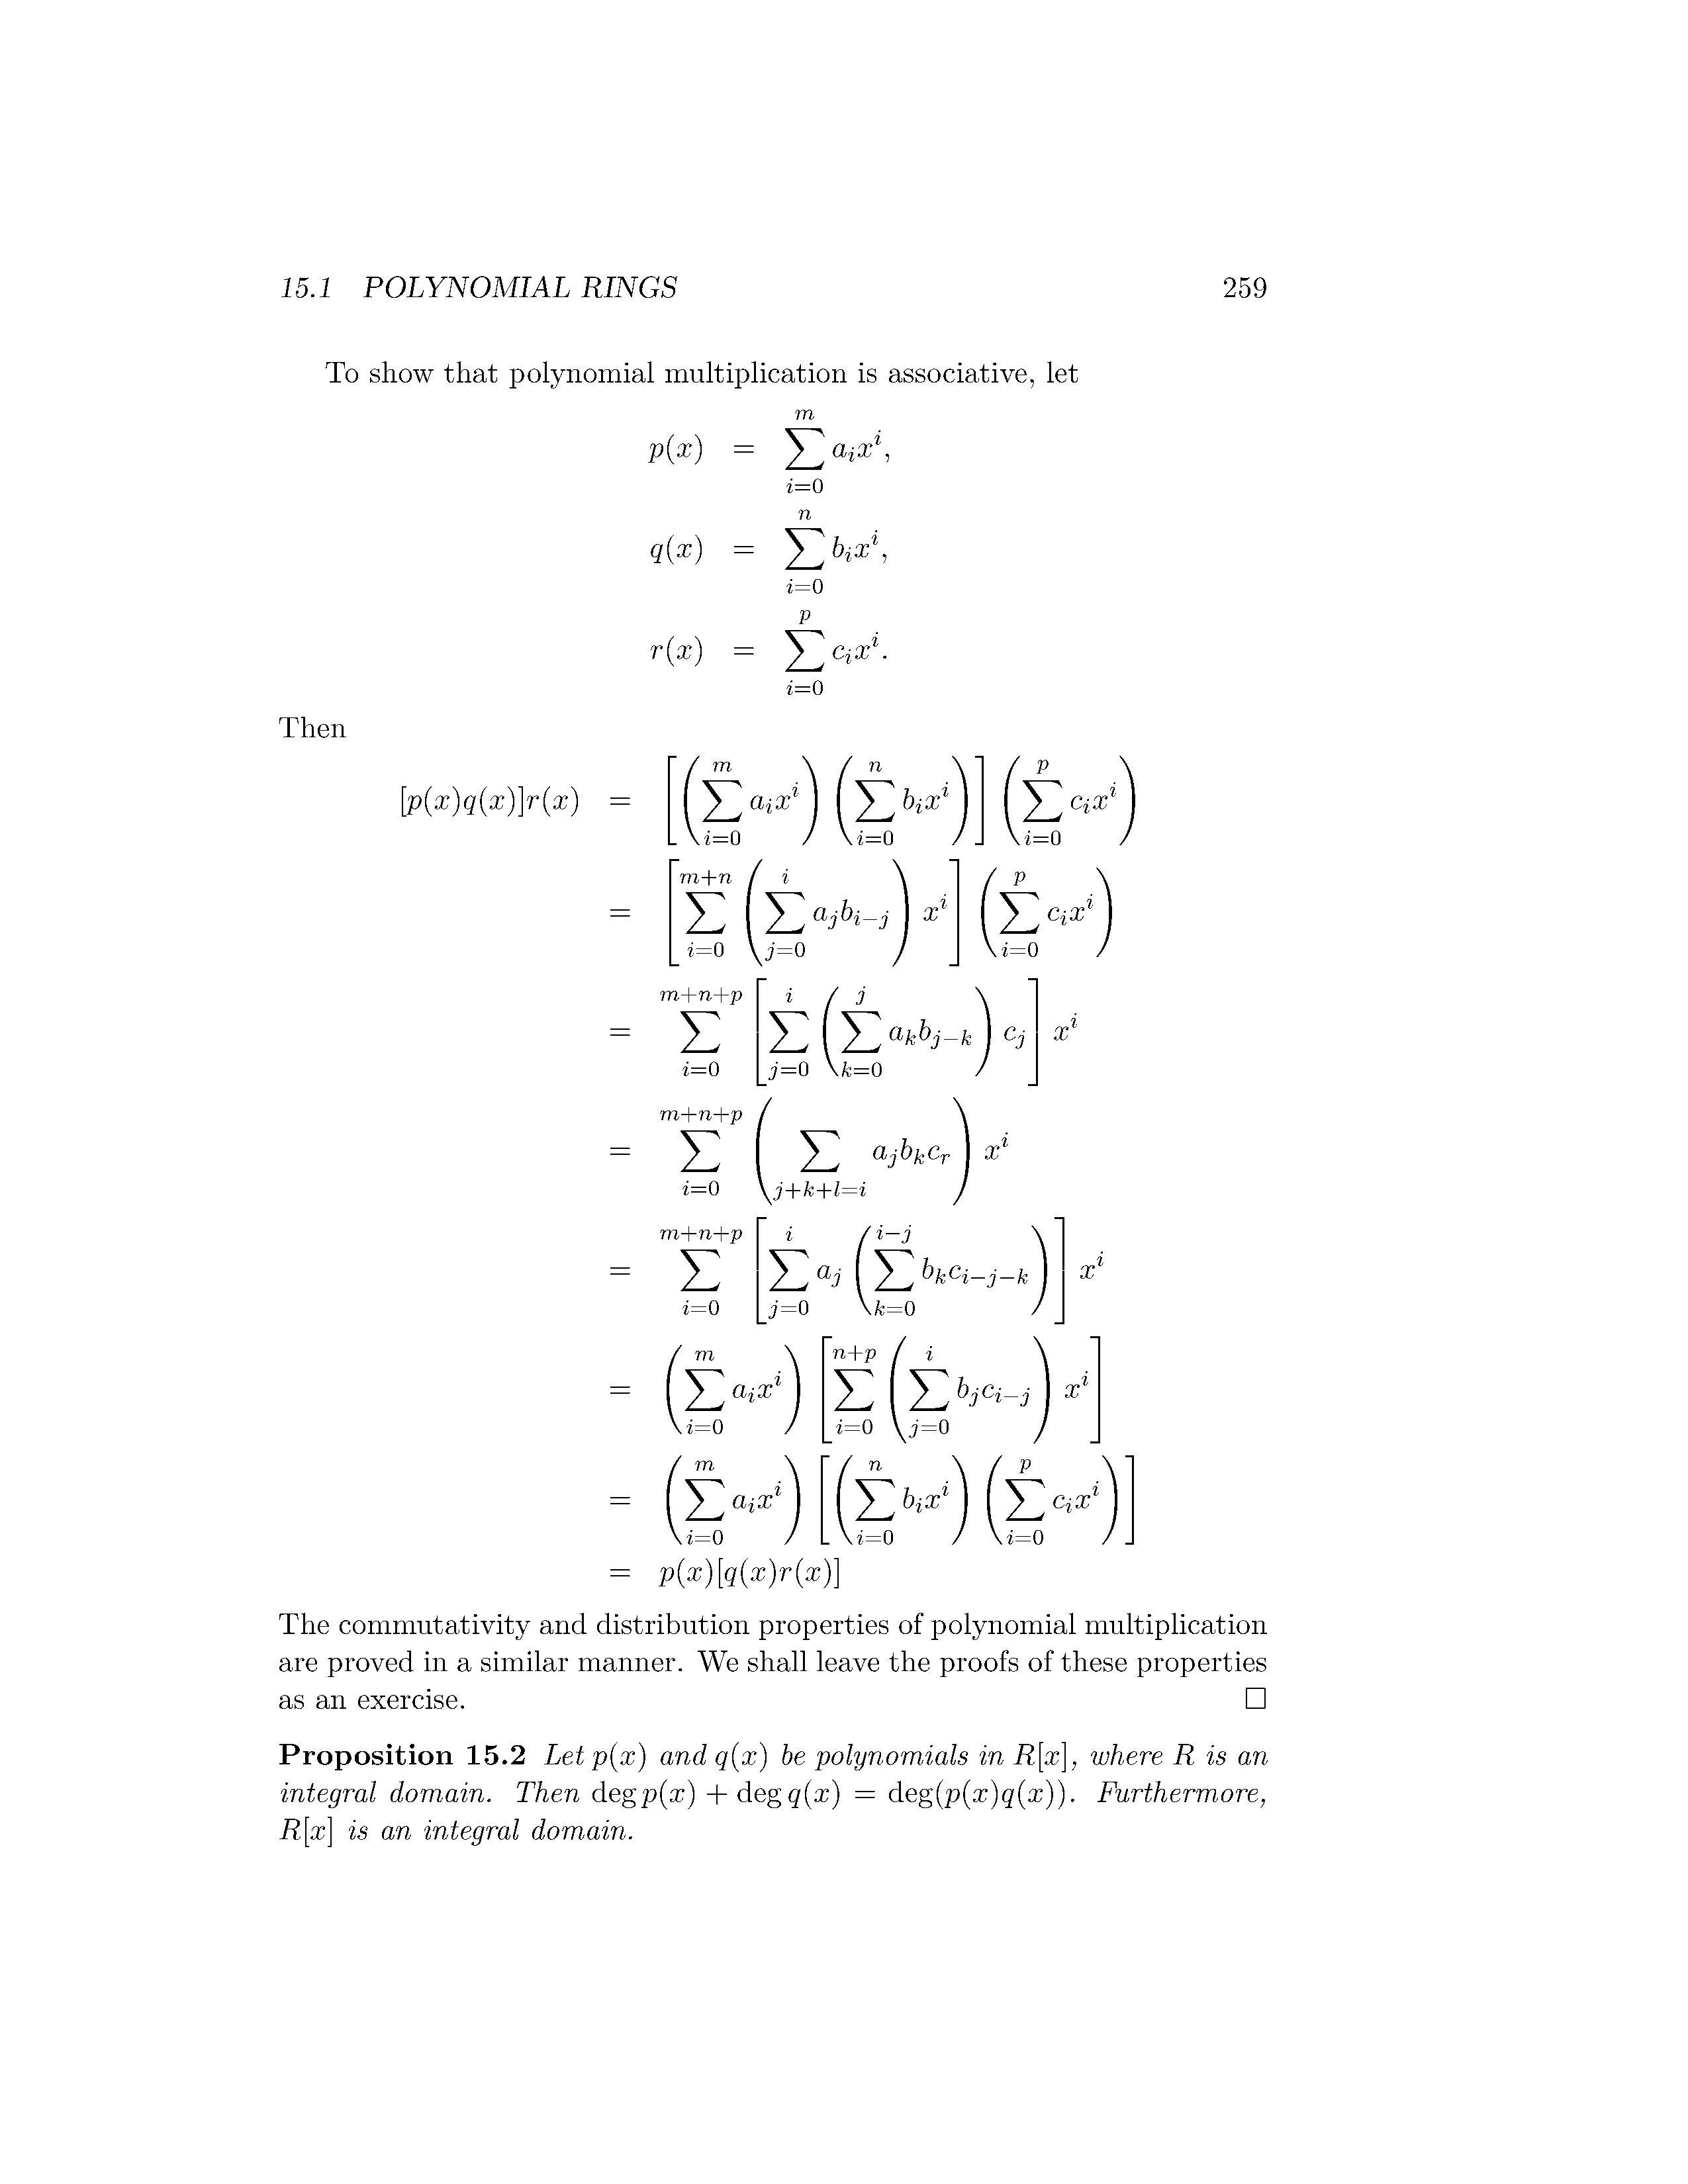
\includegraphics[width=1.0in, height=1.3in]{org.png} &
 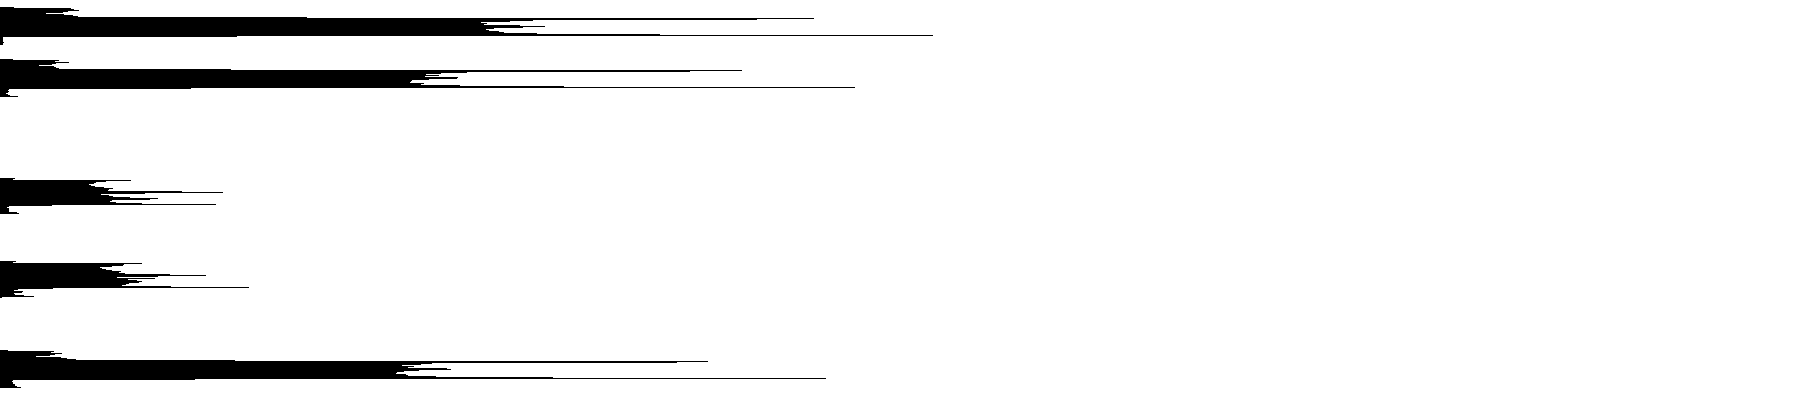
\includegraphics[width=1.0in, height=1.3in]{hProj.png} \\ 
 (a) Image &(b) Horizontal Projection Profile
 \\\hline
 \end{tabular}
 \caption{A document page and its horizontal projection profile}
 \label{hproj}
\end{figure}
 
 \subsection{Creation of word blobs in Text lines}
 This is done by merging the characters in a word. Such character coalescing process depends on the accuracy in detecting the normal
character gap and the gap between the consecutive connected components in that text line.

The mathematical formulation for  blob formation is as follows.
Consider a binary image $I_{P \times Q}$, which consists of connected
components $C_k (k=1,2,\ldots ,P)$, as defined in standard text \cite{gonzalez92}
with their usual meanings.
Let $L(C_k)$, $R(C_k)$, $T(C_k)$ and $B(C_k)$
be the four corner  points of the $k_{th}$ connected component in  left, right, top and bottom
directions respectively.

\begin{figure}[h]\center\footnotesize
\begin{tabular}{|c|c|}\hline
 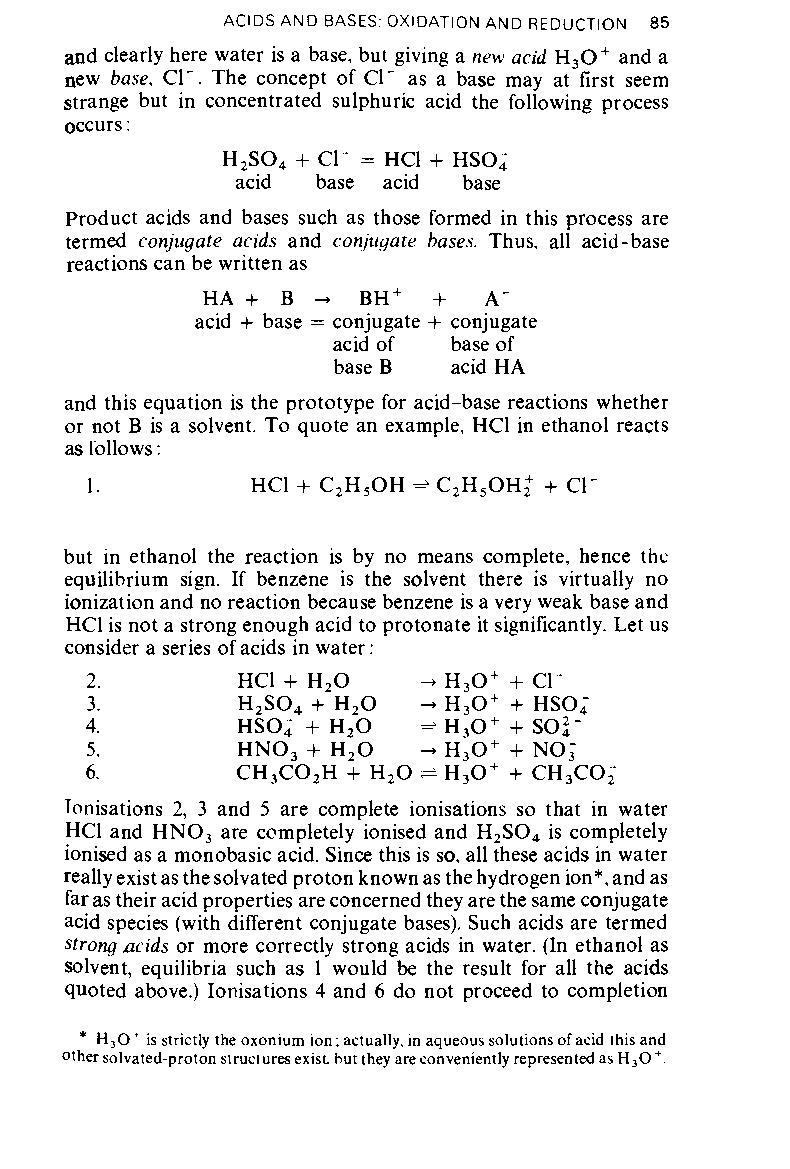
\includegraphics[width=2.0in, height = 1.5in]{page_image.png} &
 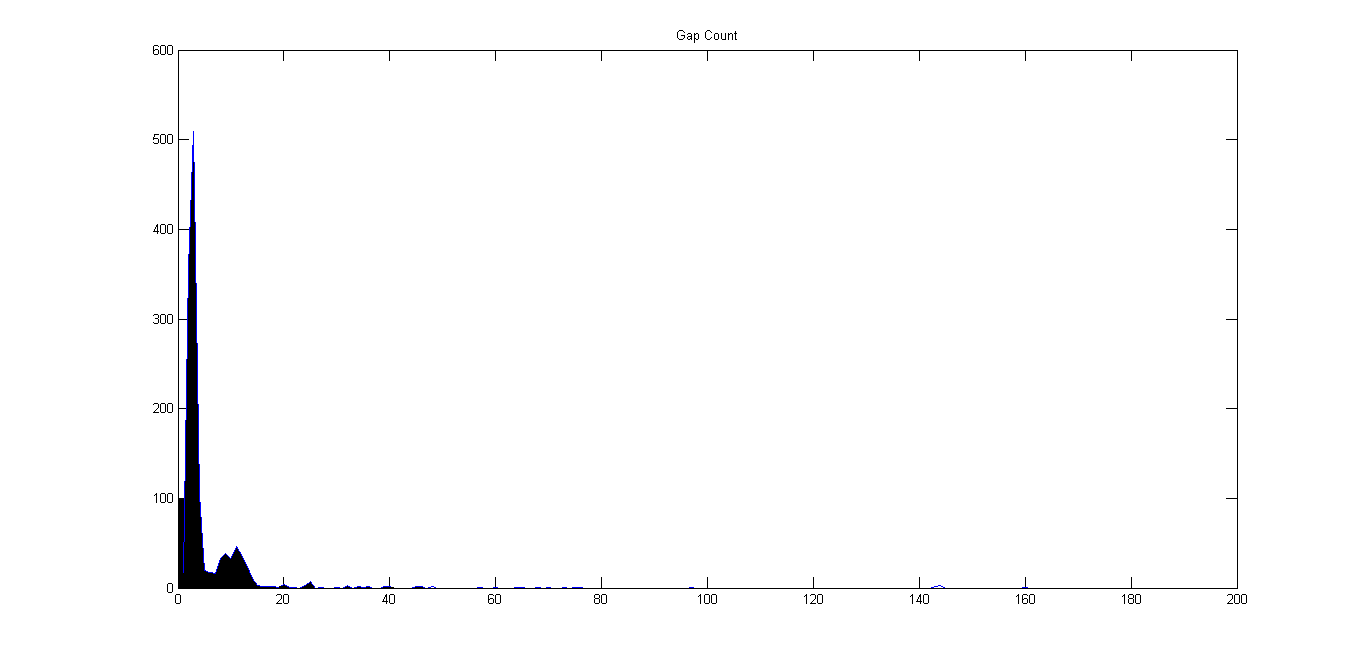
\includegraphics[width=0.5\textwidth]{cw_gap.png} \\ 
 (a)  &(b)
 \\\hline
 \end{tabular}
 \caption{Example of a page and histogram. (a) Document page (b) Histogram of the preprocessed page.}
 \label{page_histo}
\end{figure}

Let  $F$ be a function which ensures that the two connected
components lie in the same text line.
Then $F$ may be represented as
{\scriptsize
\[F(C_a,C_b)=\left\{ \begin{array}{llc}
1 & \mbox{if} & (T(C_a)\leq B(C_b)\  AND\  B(C_a)\geq T(C_b)) \\
0  & \multicolumn{2}{l}{\mbox{otherwise}}
\end{array} \right. \]
}

Cluster formation requires information on inter-word gap. 

The  distance function, D, obtained from the histogram $H_1$, is defined for computing the horizontal
distance between any two consecutive connected components $C_a$ and $C_b$, as shown below
\[D(C_a,C_b) = L(C_b) - R(C_a)\]
where $b = \min\limits_x$\{${ L(C_x) - R(C_a)}$\} such that $(F(C_a,C_x) = 1$
AND $L(C_x)>R(C_a))$.
The histogram $H_1$ registers the  gap between
two consecutive characters.
It may be noted that  there may be more than two
distinct humps in $H_1$, first one represents the character gaps in  words and the second one
represents the normal word gaps in  text lines. An example page
and corresponding histogram is shown in
Fig.~\ref{page_histo}(a) and (b).

\begin{figure}[h]\center\footnotesize
 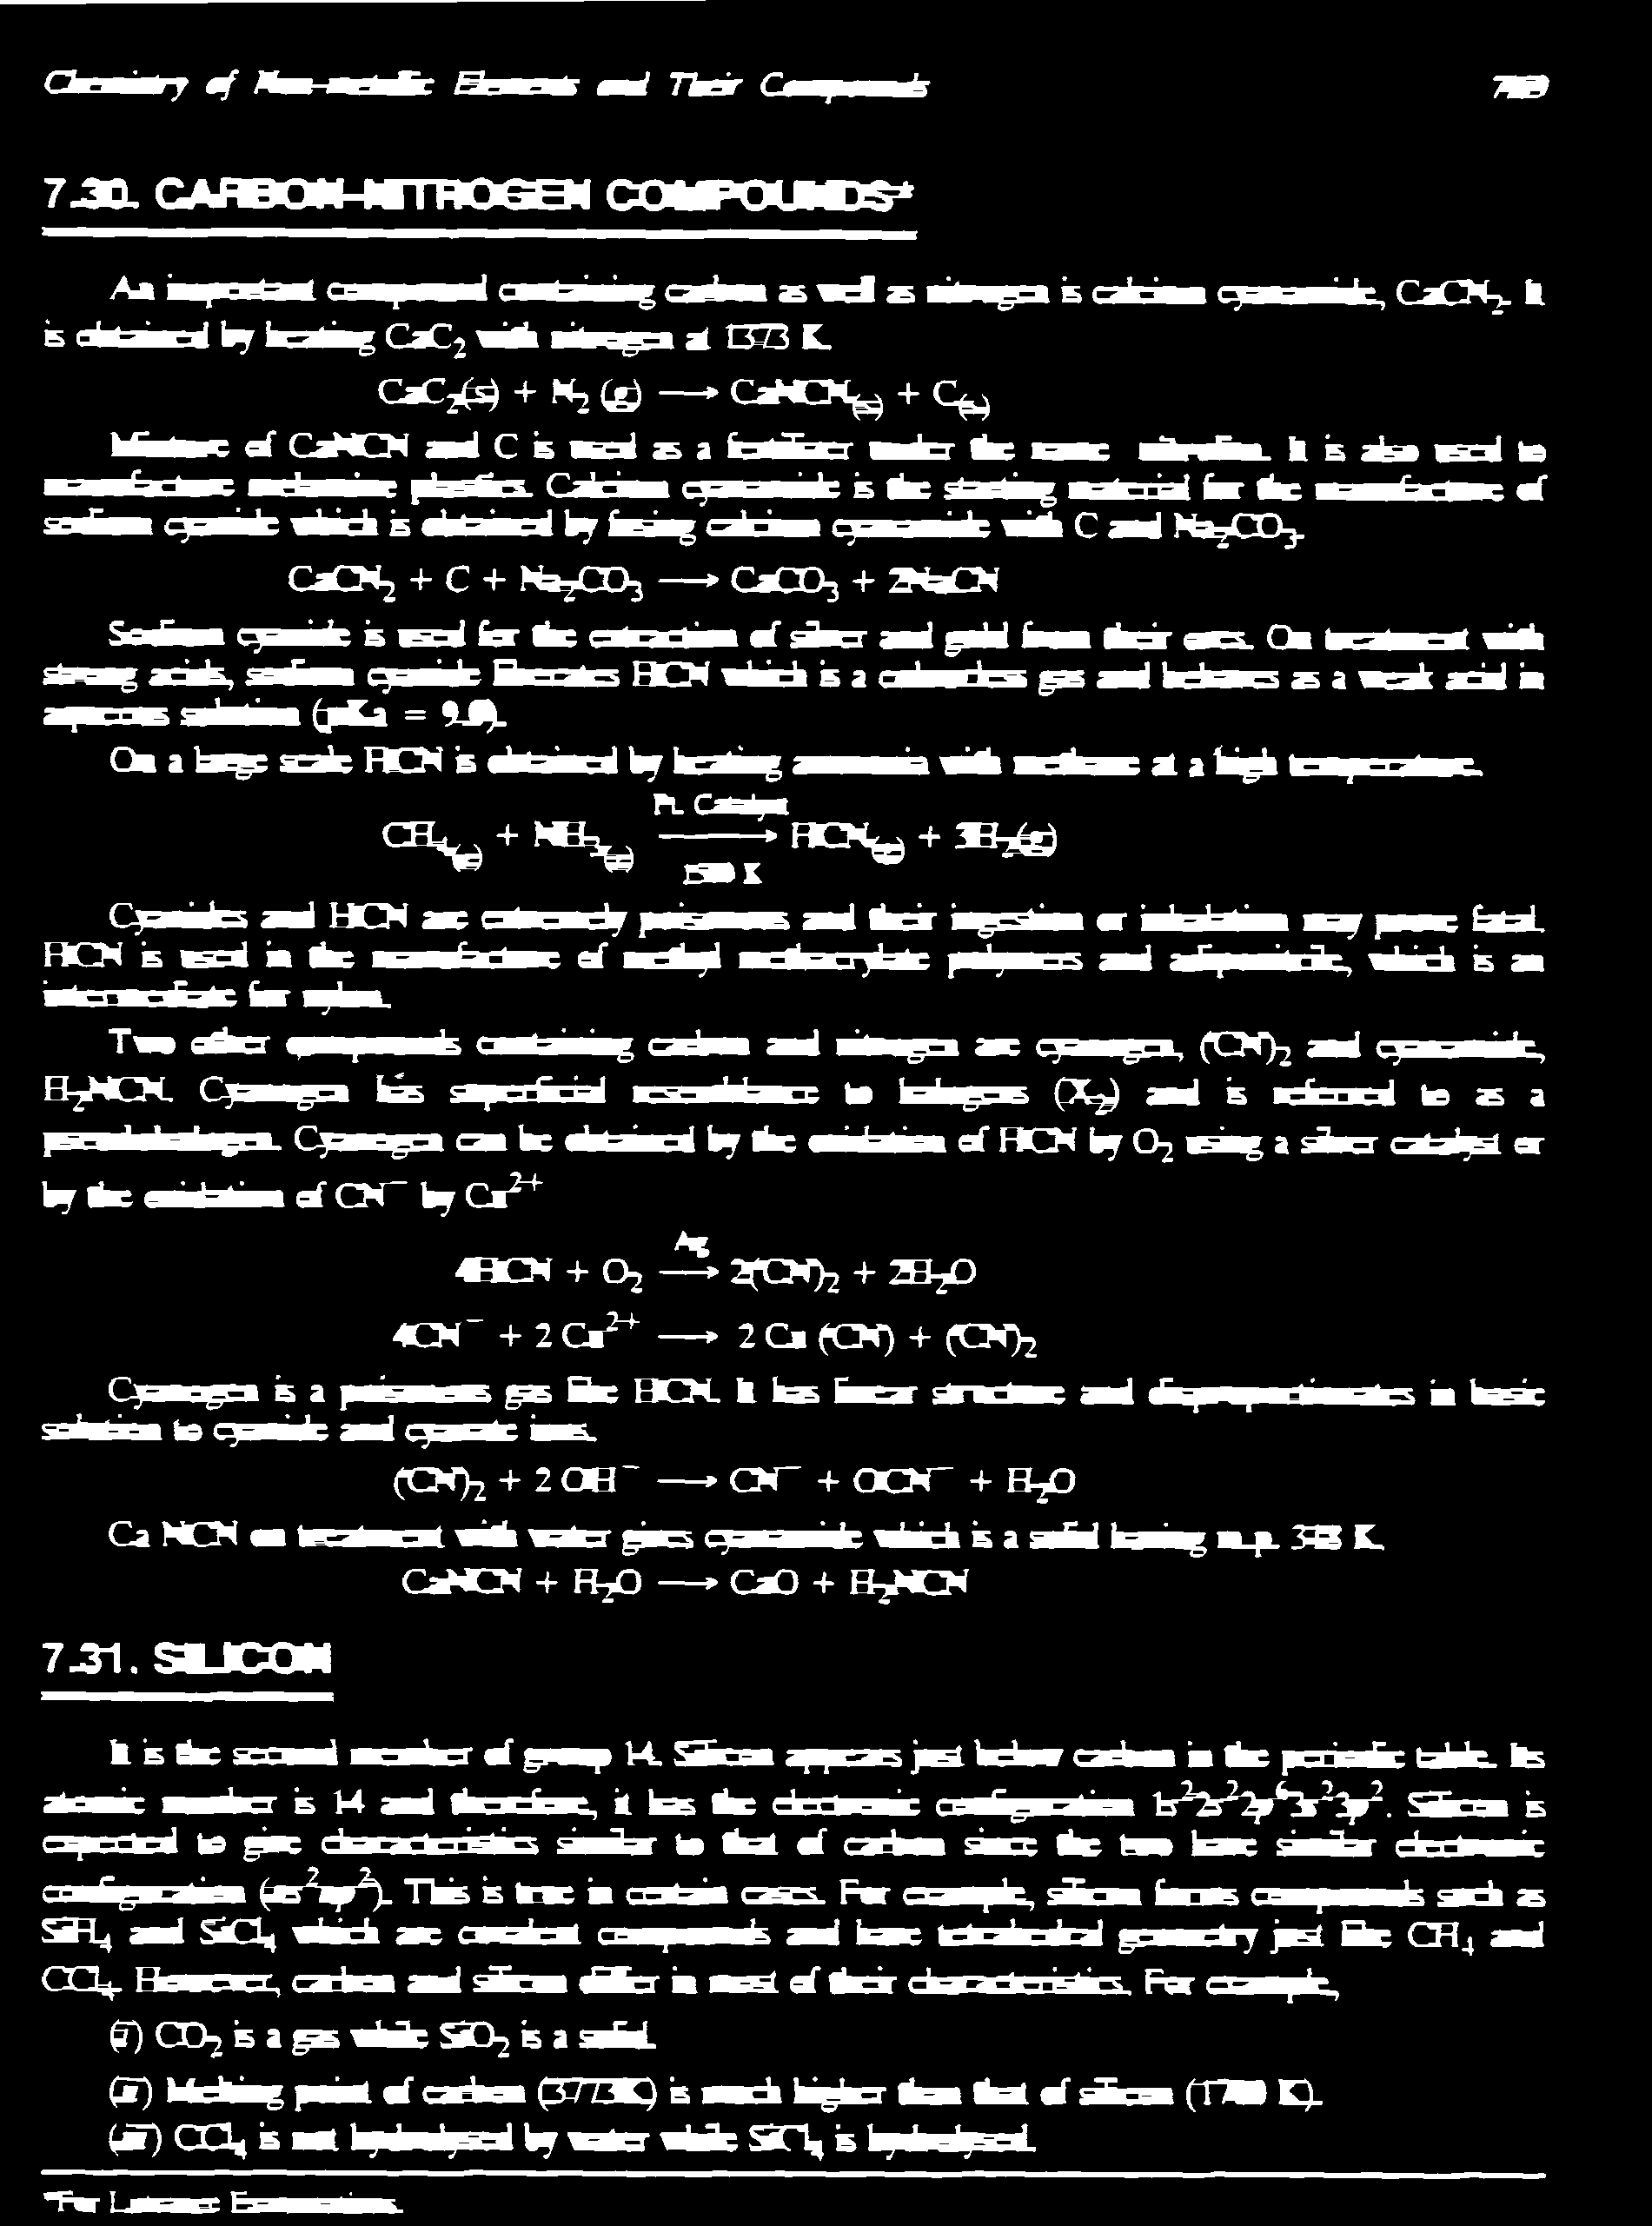
\includegraphics[width=0.4\textwidth]{wordBlob.png} 
  \caption{Example of blob formation. Clusters formed from a portion of the image shown in
Fig.~\ref{page_histo}(a).}
 \label{word_blob}
\end{figure}

Our intention is to
find out character gaps in running texts of a document page so that we could
combine the consecutive characters into a single blob. Hence, we consider
the upper boundary ($\upsilon$) of the first hump as the length of structuring
element. Morphological
close operation with a structuring element of area
$\ (\upsilon \times \ 1)$ will form the blobs denoted as
$V_w$ (where $w\ =\ 1,2,\ldots ,Q$). The
blob formation will be dictated by the following
two conditions:
\begin{enumerate}
\item If there are two connected components $C_m$ and $C_n$ $\ (1\leq m,n\leq P)\ $
obeying the relations
\begin{itemize}
\item $ \ F(C_m, C_n) = 1 $
\item $ D(C_m, C_n) \leq \upsilon $
\end{itemize}
then $C_m$ and $C_n$ should belong to the same blob.
\item $ V_a \cap V_b = \emptyset \ \ \forall \ a,b \ | \ (1\leq (a,b) \leq Q \ \ AND \ \
 a \not= b)$
\end{enumerate}


\subsection {Operator  identification}
\label{op_id}
We have considered the set of operators that is commonly used both in  chemical equations as well as mathematical 
equations to fulfil our aim to classify displayed zones containing chemical and non-chemical equations.

\begin{figure}[htb]\center\footnotesize
\begin{tabular}{|c|c|c|}
\hline
Operators & horizontal projection & vertical projection\\ \hline

\includegraphics[width=0.2in, height=0.2in]{plus.png} &
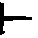
\includegraphics[width=0.2in,height=0.2in ]{plusH.png} & 

\includegraphics[width=0.2in,height=0.2in]{plusV.png}\\ \hline

\includegraphics[width=0.2in, height=0.02in]{minus.png} &

\includegraphics[width=0.2in,height=0.02in ]{minusH.png} & 

\includegraphics[width=0.2in,height=0.02in]{minusV.png}\\ \hline
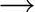
\includegraphics[width=0.2in, height=0.05in]{arrow.png} &
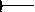
\includegraphics[width=0.2in,height=0.05in ]{arrowH.png} & 

\includegraphics[width=0.2in,height=0.05in]{arrowV.png}\\ \hline
\end{tabular} 
 \caption{Operators and their horizontal and vertical projection profiles}
 \label{h_v_profile}
\end{figure}
\begin{figure}[h]\center\footnotesize
\begin{tabular}{|c|}\hline
 
\includegraphics[width=0.5\textwidth]{singleChar.png} \\\hline
 \end{tabular} 
 \caption{Sigle components extracted from the word blobs shown in Fig.~\ref{word_blob}}
 \label{single_char}
\end{figure}

\begin{figure}[h]\center\footnotesize
\begin{tabular}{|c|}\hline
 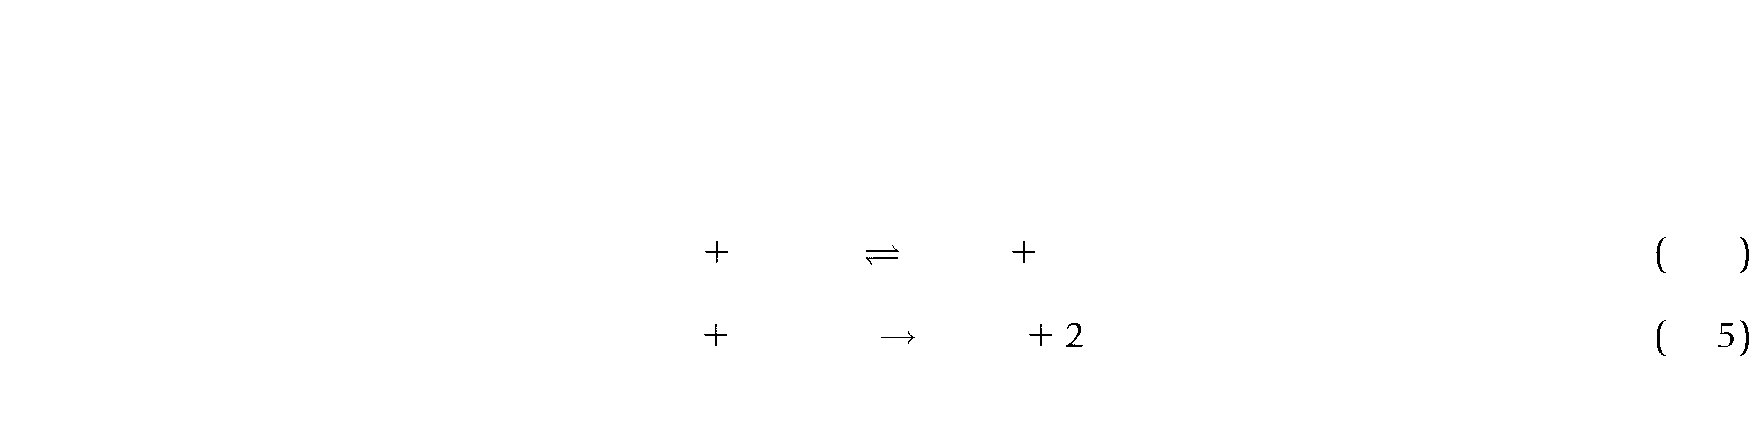
\includegraphics[width=0.6\textwidth]{singleCharafterEuler.png} \\\hline
 \end{tabular} 
 \caption{After removal of alphanumerals based on Euler number from the image shown
in Fig.~\ref{single_char}}
 \label{after_euler}
\end{figure}

\begin{figure}[h]\center\footnotesize
\begin{tabular}{|c|}\hline
 
\includegraphics[width=0.6\textwidth]{operator.png} \\\hline
 \end{tabular} 
 \caption{Operators extraceted from the image shown in Fig.~\ref{after_euler}}
 \label{operator}
\end{figure}

The remaining components in the blob image are operators along with some alphanumerics like $‘a’$, $‘A’$, $‘(’$, etc. The logical AND operation is performed between the blob image and the original image. The Euler number of the operators that we have considered is 1 (one) and based on this feature some of the alphanumerics are discarded. This image is denoted by $I_s$.
Width ($w$) and height ($h$) of each component in $I_s$ are determined. The components  are divided into two classes based on the ratio of $w, h$;
(i) {\em thin class} ($\frac{w}{h}$ $> 2$) and (ii) {\em regular class} ( $0.8 <$ $\frac{w}{h}$ $< 1.3$). 
Some instances of the \emph{thin}  and \emph{regular classes} are (-,  $\rightarrow$, $\leftarrow$, $\leftrightarrow$,  $\rightharpoonup$, $\leftharpoondown$, $\sim$, etc.) and  ( +, $\bullet$, X $\times$, etc) respectively. 

The number of \emph{on pixels}($N_p$) and number of \emph{off pixels} ($N_w$) within each bounding box of the thin components are calculated. 
Morphological opening operation is performed on {\em thin class} with a line like structuring element (SE) of length $\frac{w}{2}$.
If the output of the opening operation has a single component, then  thinning is performed on the corresponding original component.
Next, the number of end points of each thinned component is checked, if the number of end points is two  and $\frac{N_p}{N_w} > 0.8$, then the component under test is a `-' sign. If the number of end points is greater than two, then  element is an arrow. We need to identify the direction of the arrowhead for its correct representation in  \LaTeX\ file. The direction of arrowhead is identified by measuring the height of the arrow element near its two ends. 

From the \emph{regular class} our objective is to identify the `+' sign
and it is detected using the following rules: \\
(i)  Horizontal and Vertical Projection Profile of each component is considered;\\
(ii) Ratio of  $maxProj$, $D$ and ratio of $maxIndex$, $(M_l)$
%$\frac{maxProj}{D}$ and ratio of $\frac{maxIndex}{(M_l)}$
are obtained where maxProj is the maximum horizontal or vertical projection value, maxIndex is the index of maxProj closest to $M_l$ and D is width (height) for horizontal (vertical) profile. Here, $M_l$ is y (x) coordinate of the middle point for  horizontal (vertical) profile. 
If  $0.9 < \frac{maxProj}{D} \leq 1$,  $0.9 < \frac{maxIndex}{M_l} \leq 1.2$ and $\frac{N_w}{N_p} > 3$, then the component under test is a `+' sign.
Where $N_w$ and $N_p$ are number of \emph{on pixels} and \emph{off pixels} along the 
diagonal direction of the bounding box of the component. All the threshold values used  here are selected based on our empirical study on 234 images.


To detect `=' or `$\rightleftharpoons$' one extra step is required. 
The operators having $f_a$ $\leq$ 0.6 are considered to be thin symbols (-,$\leftharpoondown$,$\rightharpoonup$,$\rightarrow$,$\leftrightarrow$). 
 For each symbol denoting thin operator, a rectangular mask is placed below the
symbol to check if there is another one within the mask; if present the two thin operators are considered to form
an `=' or `$\rightleftharpoons$' sign. Let the length of the thin operator be $l$. The area of the  mask is  ($l \times l/2$).

The horizontal line separating  the numerator and the denominator is identified by its length which is greater than
the median length of the operators. Two windows are placed above and below  the separating line to merge all
the components within the windows with the separating line to form a single logical line. Otherwise, they would be
treated as three consecutive text lines and we will not be able to associate the intermediate math-symbols (`+', `-', `=')
 to a single expression. The area of the window is (length of the separating line) $\times$ (twice the median height of the text
lines).


\subsection{Segmentation of DE zones}
Initially, all the text lines consisting of at least one operator are considered as candidate displayed equations (CDE).
The operators are eliminated from CDE. The upper boundary ($u_v$) of the second hump of the histogram $H_1$ is obtained
which represents the word gaps in the text line. For each CDE zone Run Length Smoothing Algorithm  in horizontal direction (  H-RLSA) is 
carried out. If the distance between two neighbouring
components is less than $u_v$, it means they belong to a same word and thus are merged by H-RLSA.
H-RLSA has a similar effect as of dilation of black areas in horizontal direction. The characters
in a word are dilated and get linked/connected to the other characters of the same word. The output of
H-RLSA is shown in Fig.~\ref{h-rlsa}.

\begin{figure}[h]\center\footnotesize
\begin{tabular}{|c|}
\hline
 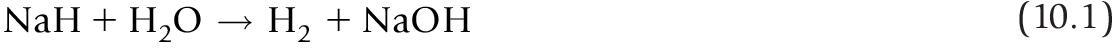
\includegraphics[width=0.6\textwidth]{line.png} \\
 (a)\\ \hline
 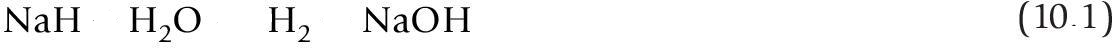
\includegraphics[width=0.6\textwidth]{linewithoutOP.png} \\
 (b) \\ \hline
 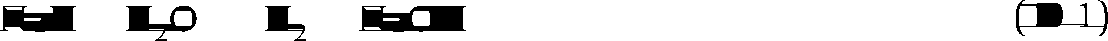
\includegraphics[width=0.6\textwidth]{lineClosed.png}\\ 
 (c) \\\hline
 \end{tabular} 
 \caption{The output of H-RLSA on portion of an image (a) a part of an image;
 (b) same part without operators; (c) result of H-RLSA operation }
 \label{h-rlsa}
\end{figure}

The equation number is common in the displayed equation zone. This has to be removed because for each CDE
we have counted the number of operators  and corresponding other components  in the output of H-RLSA. If the number of components 
 $\le$ 2$\times$ number of operators, then the CDE is considered as a displayed equation;
otherwise some embedded formulas/equations may exist in the line. To eliminate the equation number from the output of H-RLSA  the operators are  moved here and the component 
analysis is done. From both ends distance ($d$) (see Fig.\ref{end_rev})between the first two consecutive components is measured and if $d$  $> 5\times$  $u_v$, 
then the first component from the end is considered as equation number and is removed.
\begin{figure}[h]\center\footnotesize
\begin{tabular}{|c|}
\hline
 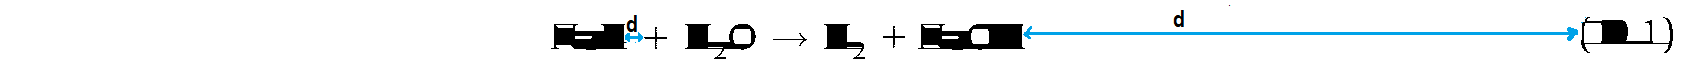
\includegraphics[width=0.6\textwidth]{endRemoval.png} \\ \hline
 \end{tabular} 
 \caption{Example of a equation number present in DE zone}
 \label{end_rev}
\end{figure}

\subsection{Experimental Results}

We have implemented our algorithm in MATLAB 8.3.0.532
(R2014a) in a PC (Intel(R) Core(TM) i5-3337U CPU @ 1.80GHz
running Windows 8). The proposed method has been tested on
a dataset consisting 234 document pages. Out of 234 pages 50
pages are taken from ICDAR 2013 Math-zone segmentation
datasets and other document pages are scanned from different Mathematics and
Chemistry books. 

%\begin{table}[h]\center\scriptsize
%\caption{ Summary of experimental results}
%\begin{tabular}{|l|c|c|c|}\hline
%                   
%\diaghead{\theadfont tableOfExperiment}%
%{Actual}{Classified\\As}&
%\thead{Chemical}&\thead{Other}\\ \hline
%Chemical & 97.8\% & 2.2\%\\ \hline
%Other & 2.95\% & 97.05\%\\ \hline
%
%\end{tabular}
%\label{tab:summary}
%\end{table}

\begin{table}[h]
\captionof{table}{Summary of Experimental Results}
\centering
\begin{tabular}{|c|c|}
\cline{1-2} 
{\color[HTML]{000000} \# Total Images}                     & 234   \\ 	\cline{1-2}
{\color[HTML]{000000} \# Total DEs}                        & 1390    \\ \cline{1-2}
{\color[HTML]{000000} DE segmentation accuracy}            & 98.63\% \\ \cline{1-2}
\end{tabular}
\label{table:result}
\end{table}

\subsection{Error Analysis}

\subsubsection{Segmentation error}
 
Some chemical equations have some reactants/symbols (such as $\Delta$) just on top or bottom of the arrow   
 and in some cases they enter the bounding box of the arrow.  
  When we extract only single characters from the word blob information as mentioned in ~\ref{op_id},
 we do not get the arrow as it is no longer treated as a single character within its bounding box.
 Here the operator, arrow does not get detected and  the ratio between number of operands and number of operators exceeds 2.
 So, this is segmented as an embedded equation. See. Fig.~\ref{seg_error}(a).
 \begin{figure}[h]\center\footnotesize
\begin{tabular}{|c|}\hline
 
\includegraphics[width=0.6\textwidth]{escan3.png} \\
 (a)\\ \hline
 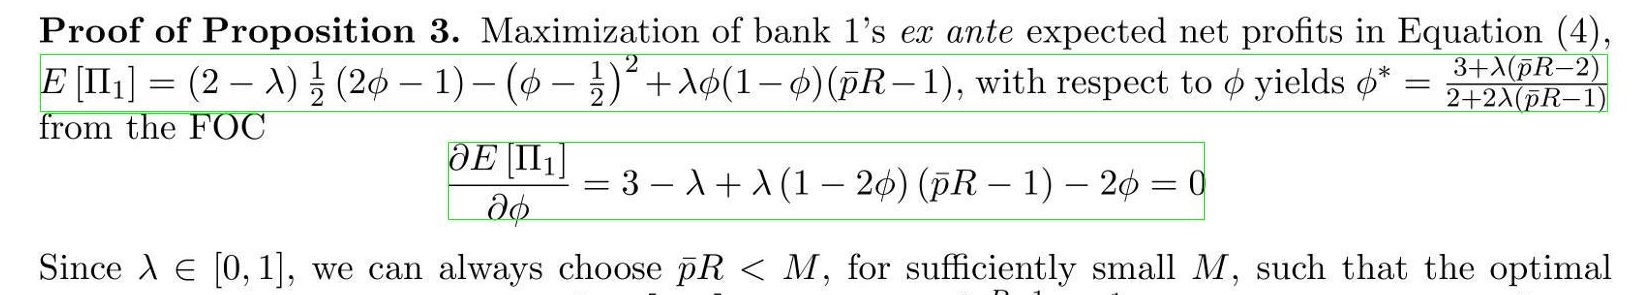
\includegraphics[width=0.6\textwidth]{chem31.jpg}\\ 
  (b)\\ \hline
  \end{tabular} 
 \caption{Examples of segmentation error}
 \label{seg_error}
\end{figure}

In a few cases, text lines consisting of embedded expressions are identified as displayed equations 
(see Fig.~\ref{seg_error}(b)), but in those cases the text lines contain more mathematics than normal text.
However, identification of mathematics intensive text lines as mathematical displayed equation is not a severe error. 

\section{Classification of segmented DE zones}

Each segmented displayed equation is divided into three zones; namely upper zone, middle zone and lower zone (see Fig~\ref{sub_super}).
To identify the three zones of a DE zone, uppermost and lowermost co-ordinates of each connected component below the same DE zone  are also obtained.
The median of uppermost coordinate, and median of lowermost co-ordinate of such components in DE zone are computed.
A horizontal line, called the baseline, is drawn through the median of lowermost coordinates of components
and this baseline separates the middle zone and lower zone of DE zone.
Similarly, the median of uppermost co-ordinate of the components in the DE zone  generates a horizontal line. This horizontal line, called top line, separates the middle and  upper zones of the DE zone.
\begin{figure}[h]\center\footnotesize
\begin{tabular}{|c|}
\hline
 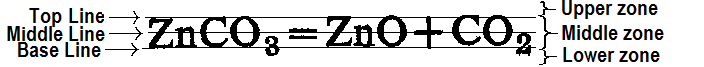
\includegraphics[width=0.5\textwidth]{s_s.png} \\ \hline
 \end{tabular} 
 \caption{Example of 3 zones present in a DE zone}
 \label{sub_super}
\end{figure}


The subscripts in a DE zone belong to lower-half of the middle zone and lower zone whereas the superscripts belong to upper zone and
upper-half of the middle zone. Based on the location of the components in a DE zone we have detected the subscripts and superscripts
and removed from the DE zone. The operators are also removed from DE zone.

Now, each displayed equation is an input to an OCR of MATLAB
R2014a.
The OCR returns each DE zone as a text string.
We made a dictionary out of all the elements in the periodic table. An important observation is that an element always starts with a capital letter. Using this property,
an element can be expressed by a regular expression [A-Z][a-z]*. 
It means an element's symbol
starts with an upper case letter and may or may not have one or more lower case letters. 
We have designed a parser to extract the sub-strings matching the above-mentioned regular expression with the following grammar:\\
\begin{center}
$start \rightarrow capital.follow$\\
$follow \rightarrow small.follow | \in$\\
$capital \rightarrow A|B| \dots |X|Y|Z$\\
$small \rightarrow a|b| \dots |x|y|z$\\
\end{center}

The working principle of the parser is depicted in Fig.~\ref{flow_chart}.
Each of the substrings returned by the parser is matched against the aforesaid dictionary and if it is a positive match then 
that substring is considered as a symbol of the chemical element. 
Let us consider, the number of substrings extracted from the OCR output by the parser is {\em n}  and the number of positive matches with 
the aforementioned dictionary is {\em m}.
If m:n ratio is more than a threshold value $\beta$ then this DE is considered as a Chemical Equation. 
This threshold ($\beta$) is set to 0.7 by running our algorithm on our dataset containing 733 segmented displayed equations. 
The reasons for $\beta$ not being 1 are
i) limitation of the OCR we used;
ii) presence of broken and touching characters in the DE zone. \par
The $\uparrow$ and $\downarrow$ are frequently used in chemical equation to represent the state of compounds and  are thus important to detect.
Let each chemical equation be denoted by $C_e$. Each $C_e$ zone is AND with $I_s$ which produces an output $I_o$. $I_o$ may contain  operators, single character elements and ($\uparrow$, $\downarrow$). The operators are removed from $I_o$ as they are already identified. For the rest of the components in $I_o$, we have checked whether the component is the starting character of the chemical equation, if not, then its immediate left neighbour in $C_e$ is checked. If the left neighbour is not an operator, then then component under test is  $\uparrow$ or $\downarrow$. The arrowhead direction is determined in the same way as right/left arrow.
\begin{figure}[h]\center\footnotesize
\begin{tabular}{|c|}
\hline
 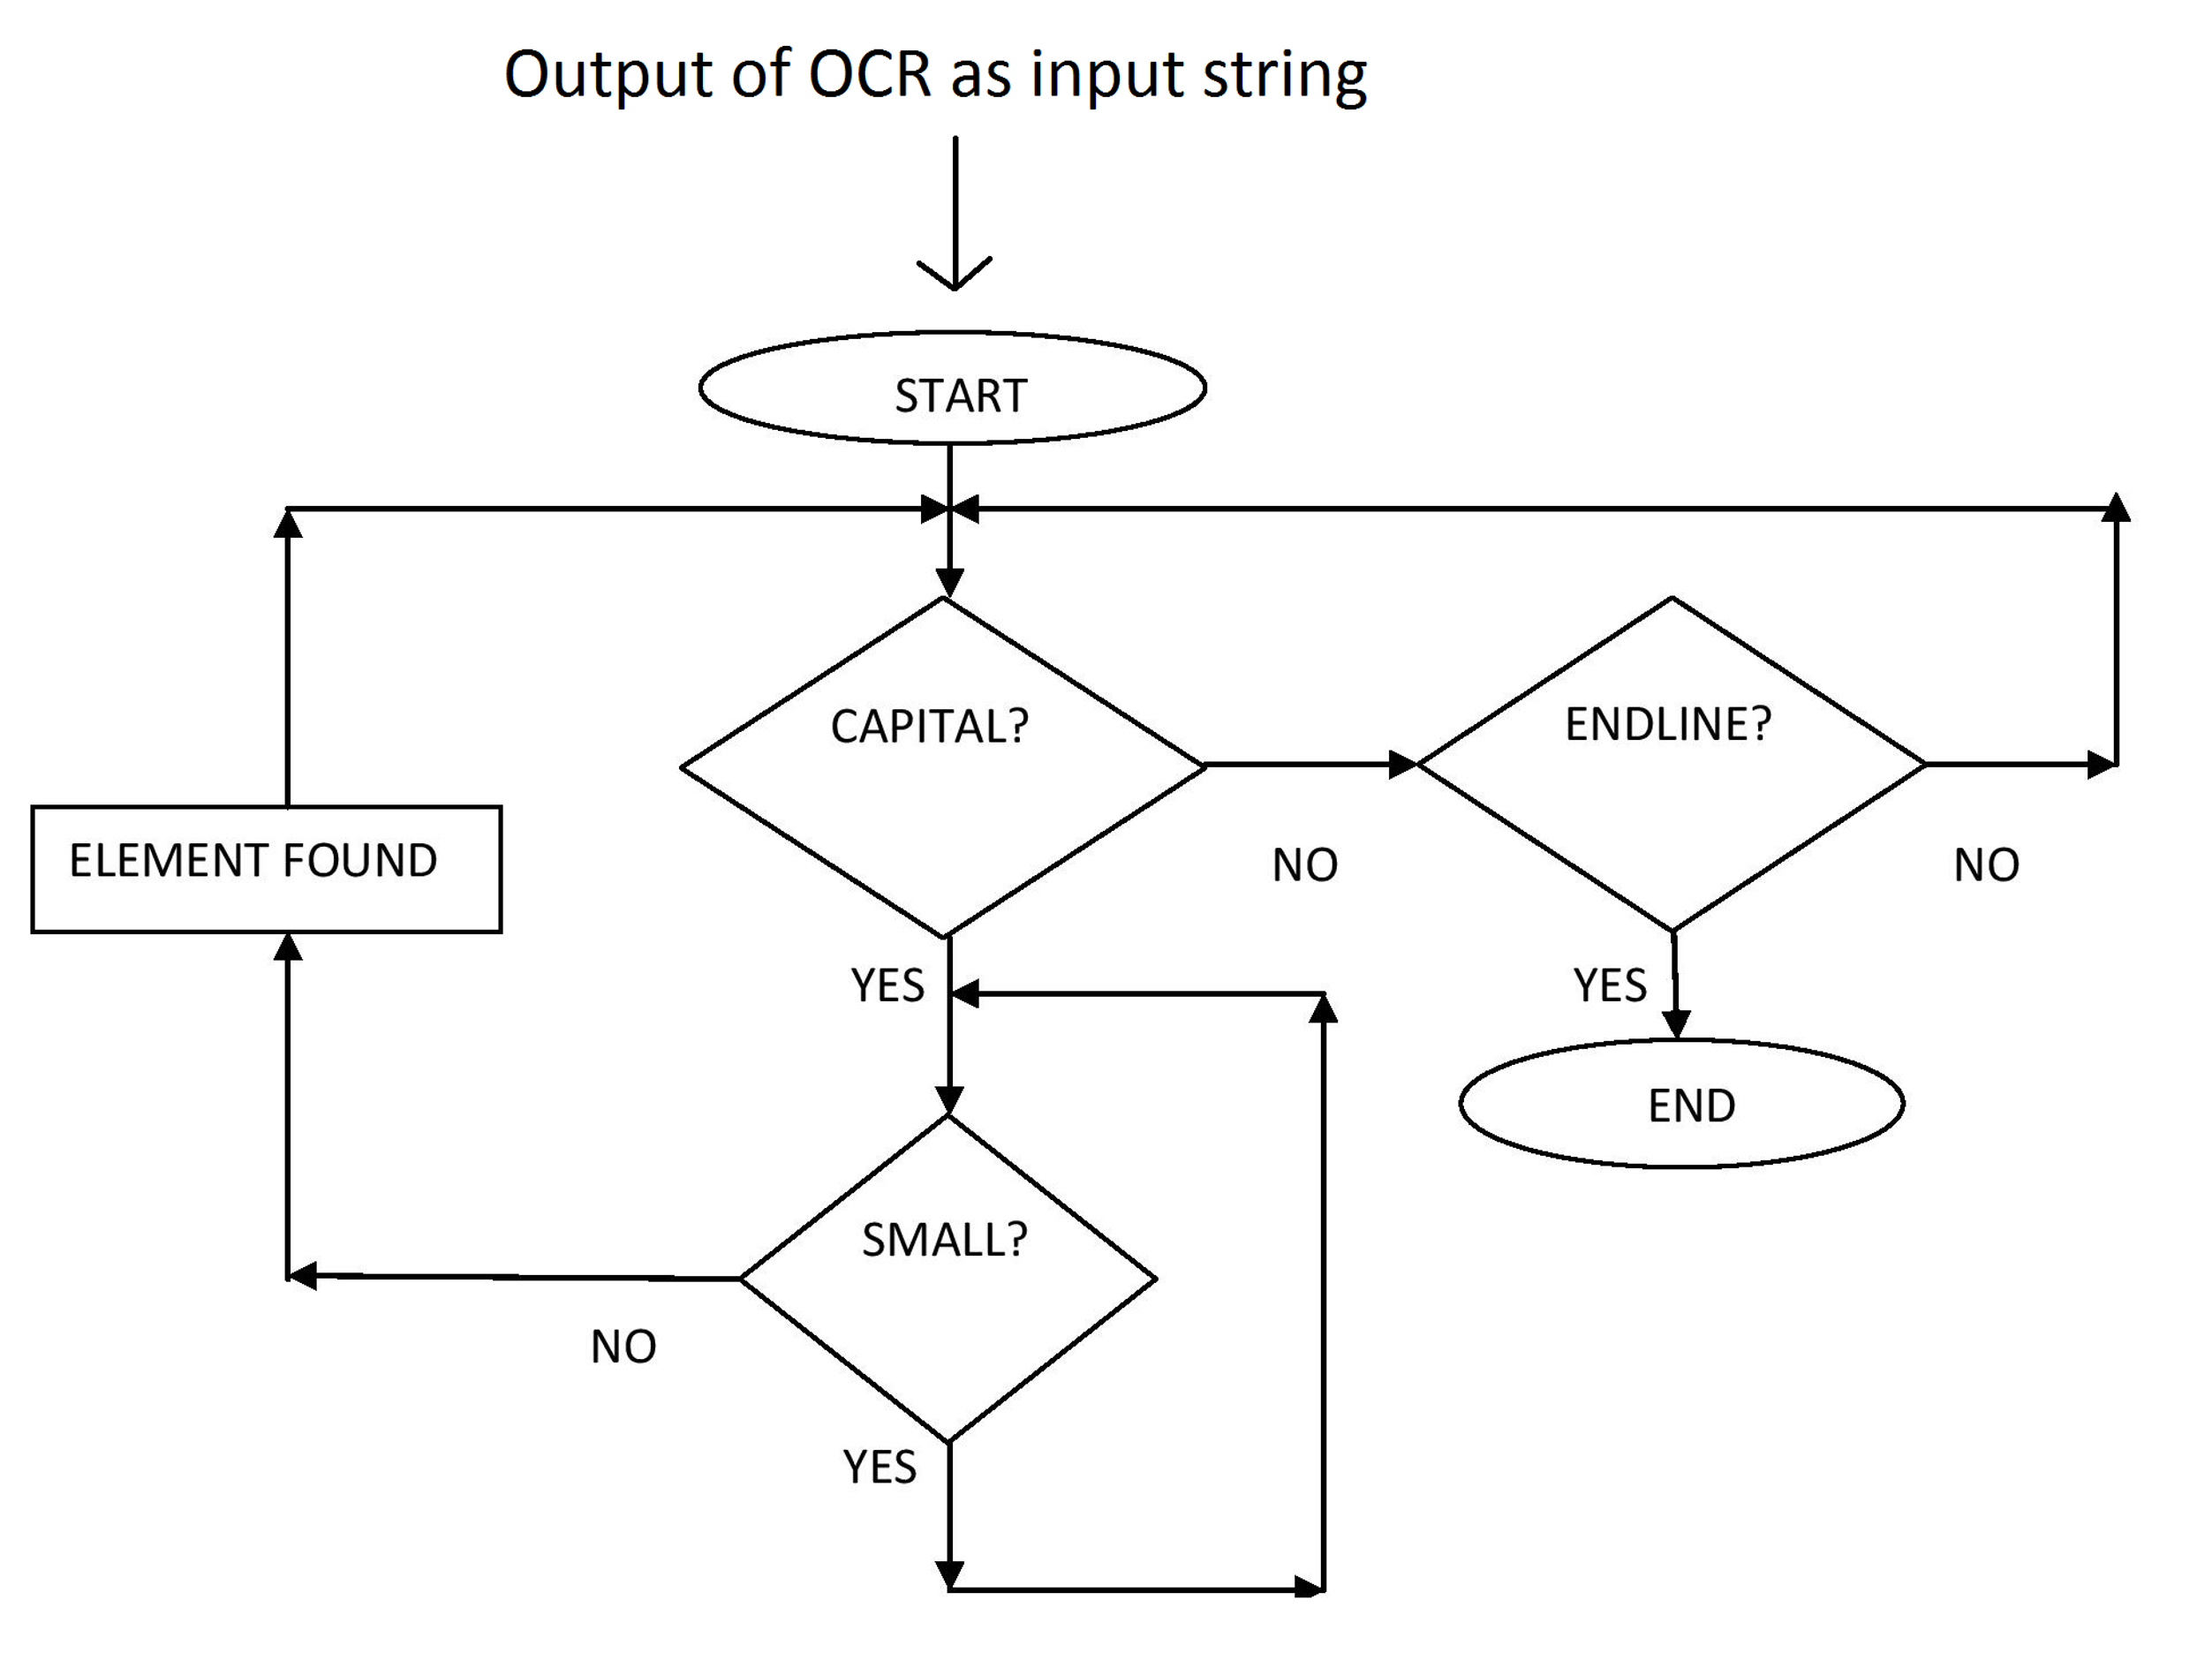
\includegraphics[width=0.6\textwidth]{flowchart.png} \\ \hline
 \end{tabular} 
 \caption{Working flow chart of the parser}
 \label{flow_chart}
\end{figure}

\subsection{Experimental Results}

We have implemented our algorithm in MATLAB 8.3.0.532
(R2014a) in a PC (Intel(R) Core(TM) i5-3337U CPU @ 1.80GHz
running Windows 8). The proposed method has been tested on
a dataset consisting 234 document pages. Out of 234 pages 50
pages are taken from ICDAR 2013 Math-zone segmentation
datasets and other document pages are scanned from different Mathematics and
Chemistry books. 

Classification outputs for some of the cases are shown in Fig.~\ref{exp_result}. In the figure  the  red and the green bounding boxes indicate chemical and 
non-chemical expressions respectively.

\begin{figure*}[!htb]\center\scriptsize
\begin{tabular}{|c|c|}
\hline
 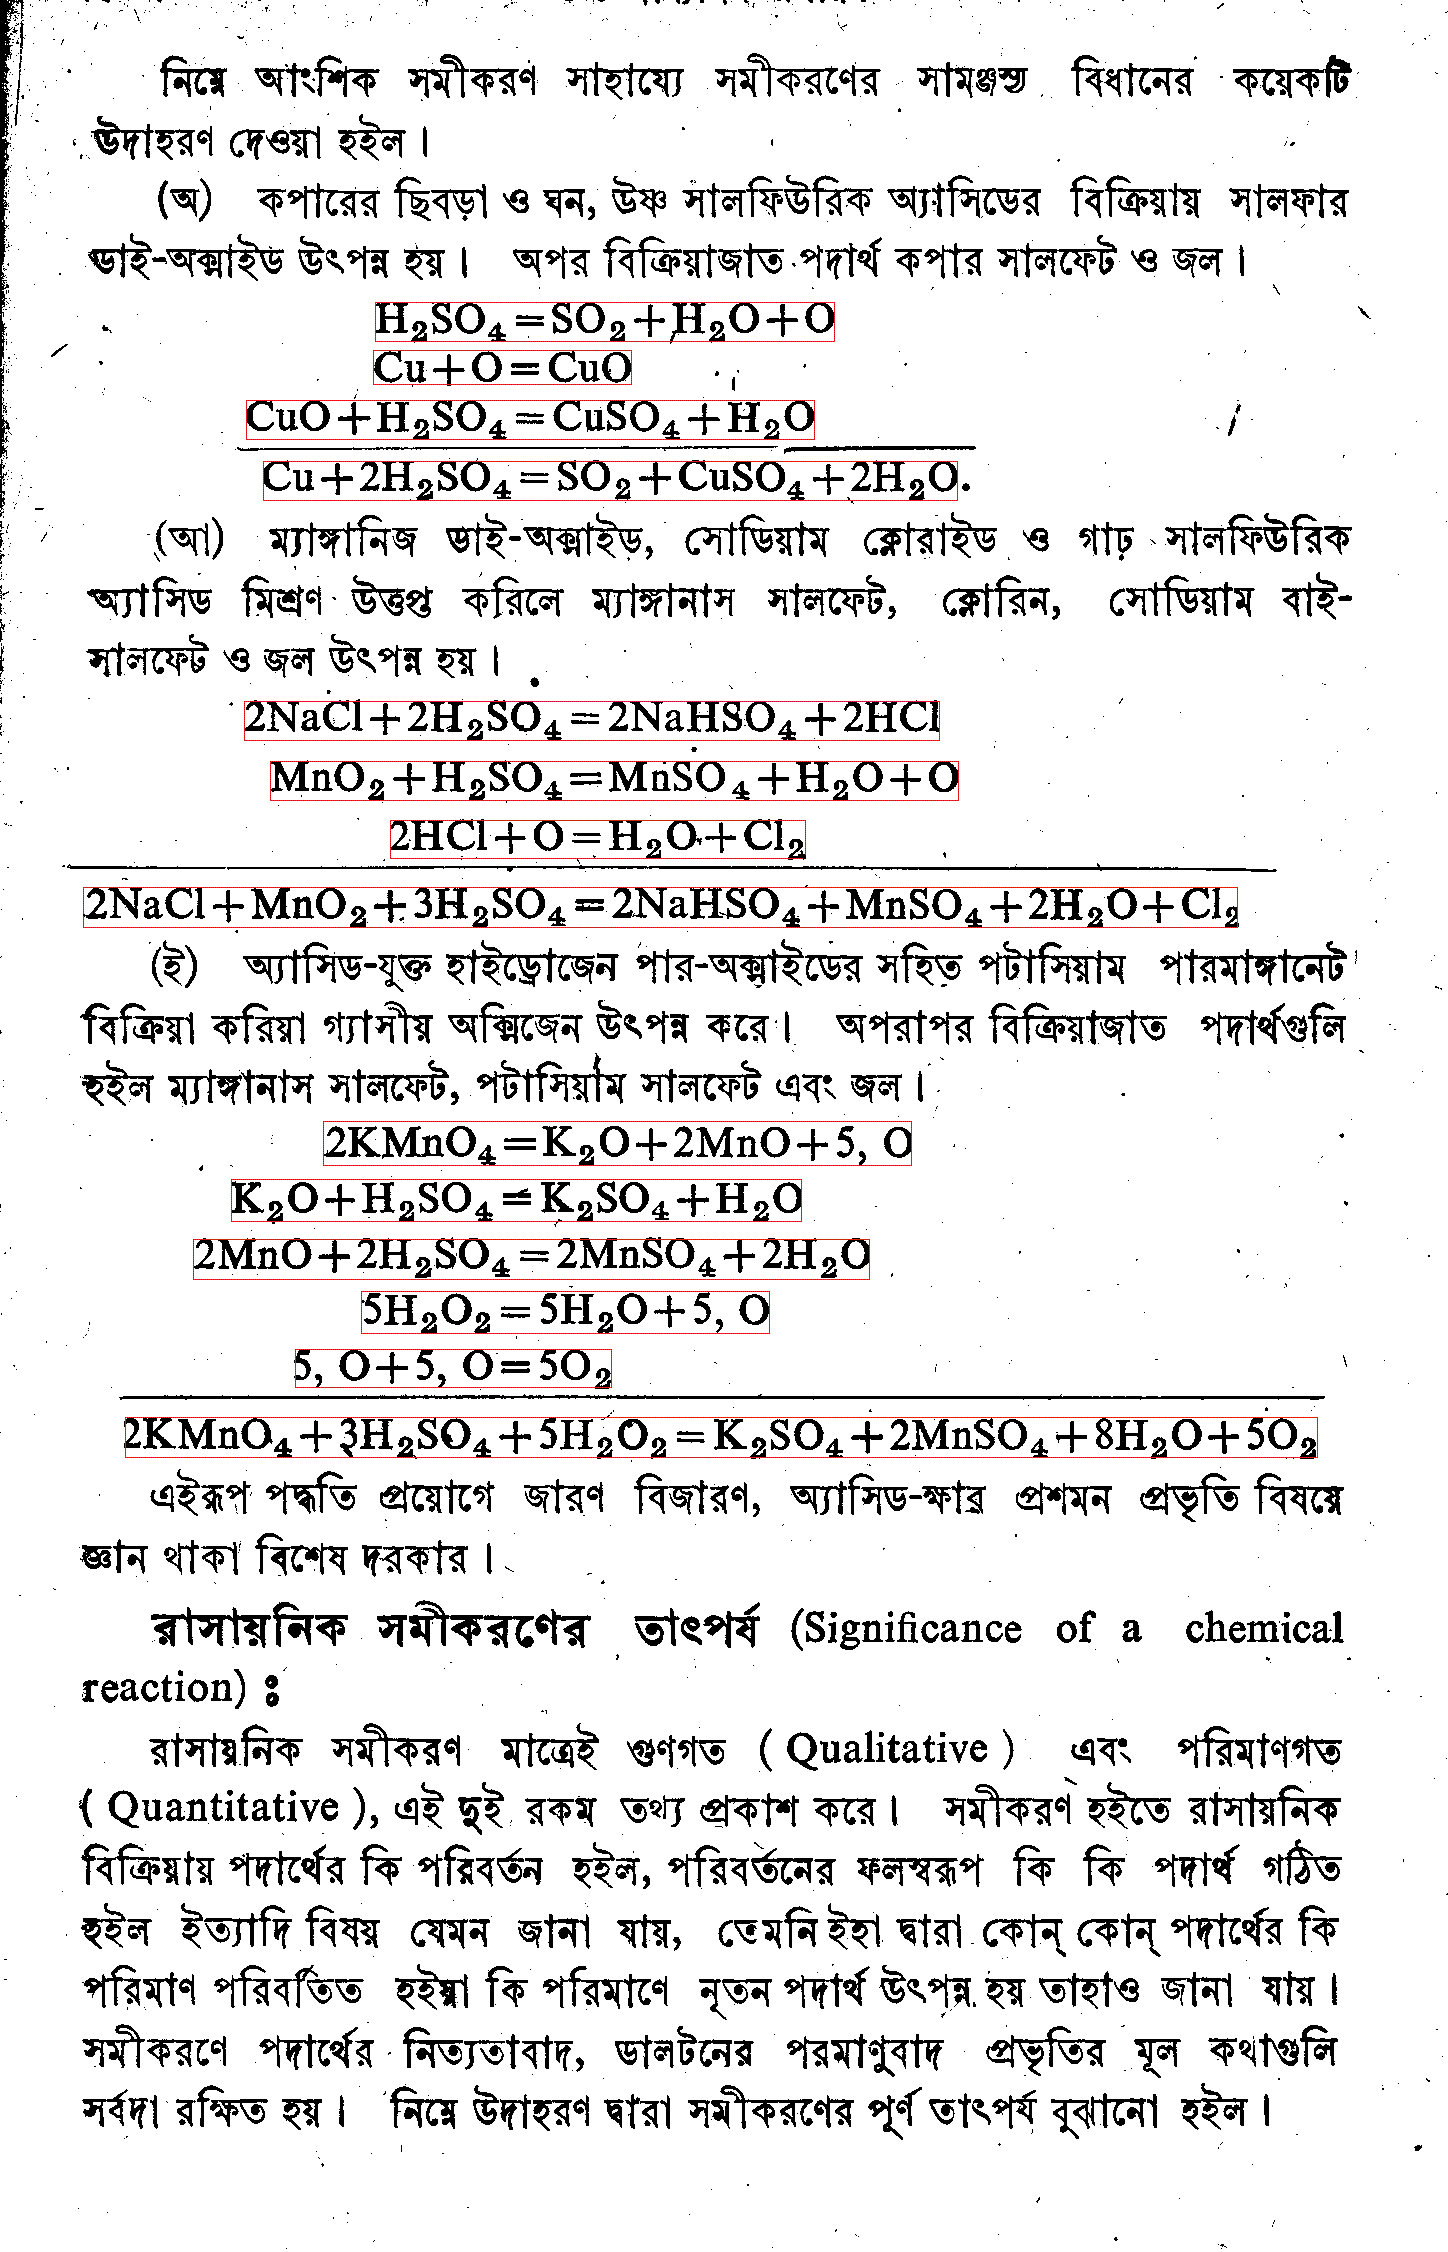
\includegraphics[width=0.42\textwidth]{result1.png} &
 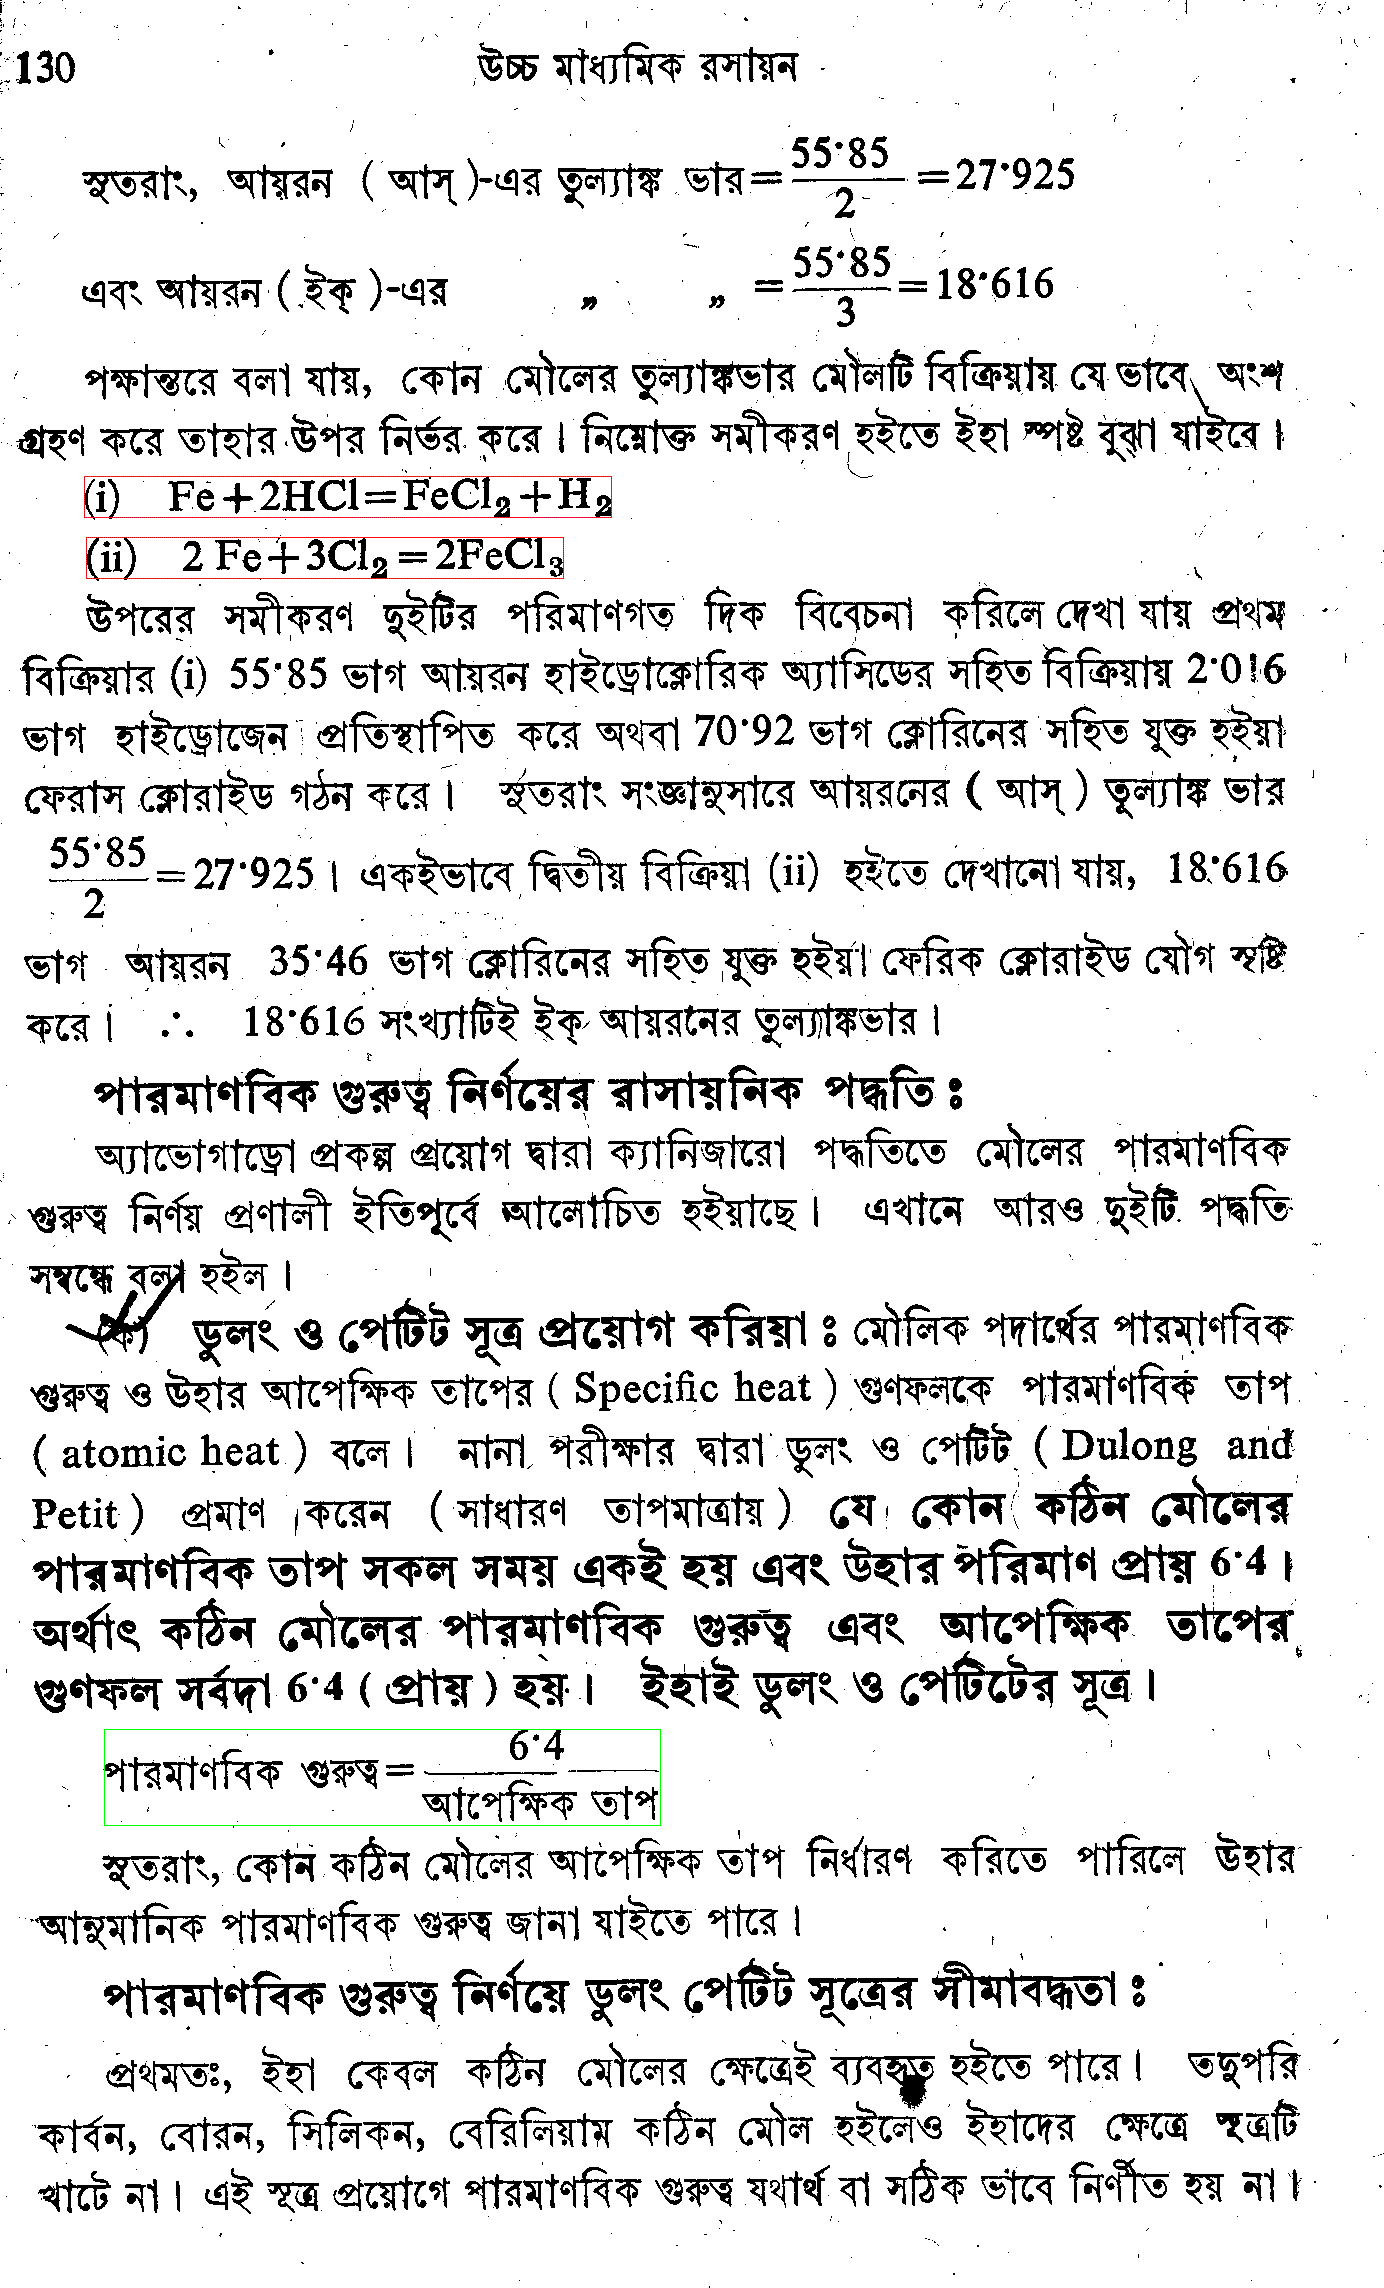
\includegraphics[width=0.42\textwidth]{result2.png} \\
 (a)  &(b)  \\
 \hline
  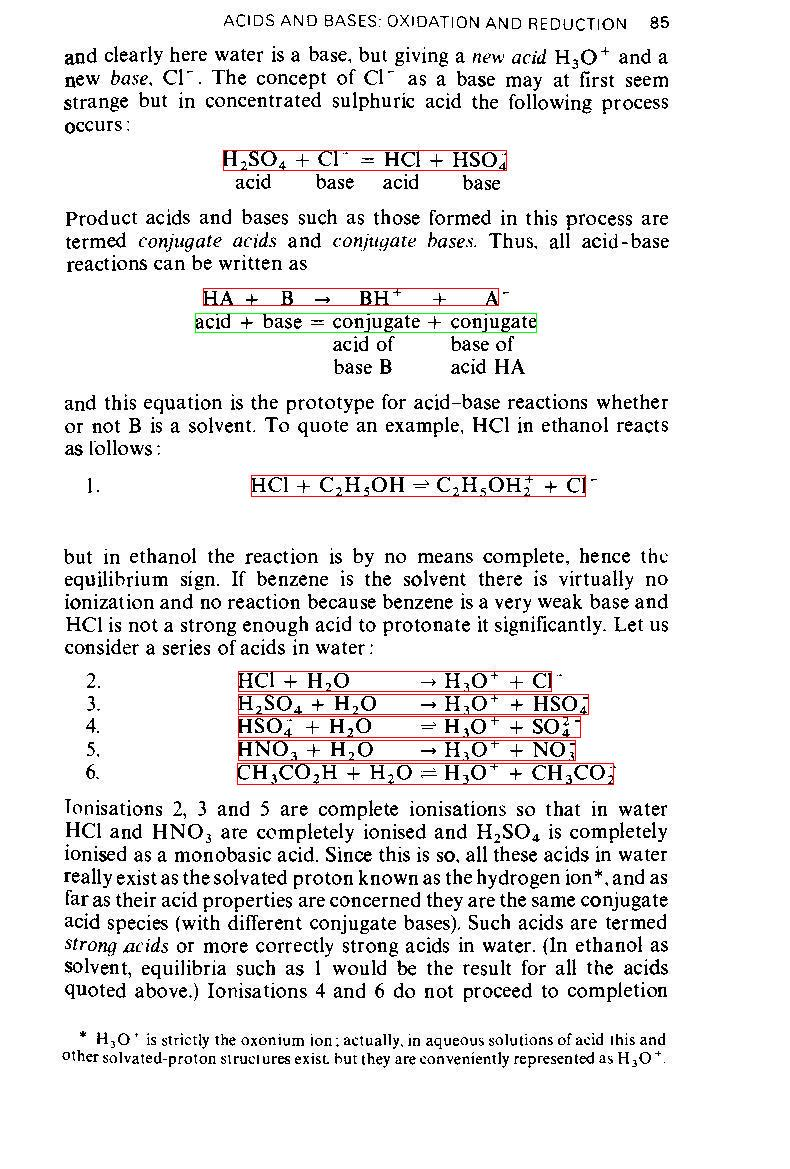
\includegraphics[width=0.42\textwidth]{result_3.png} &
 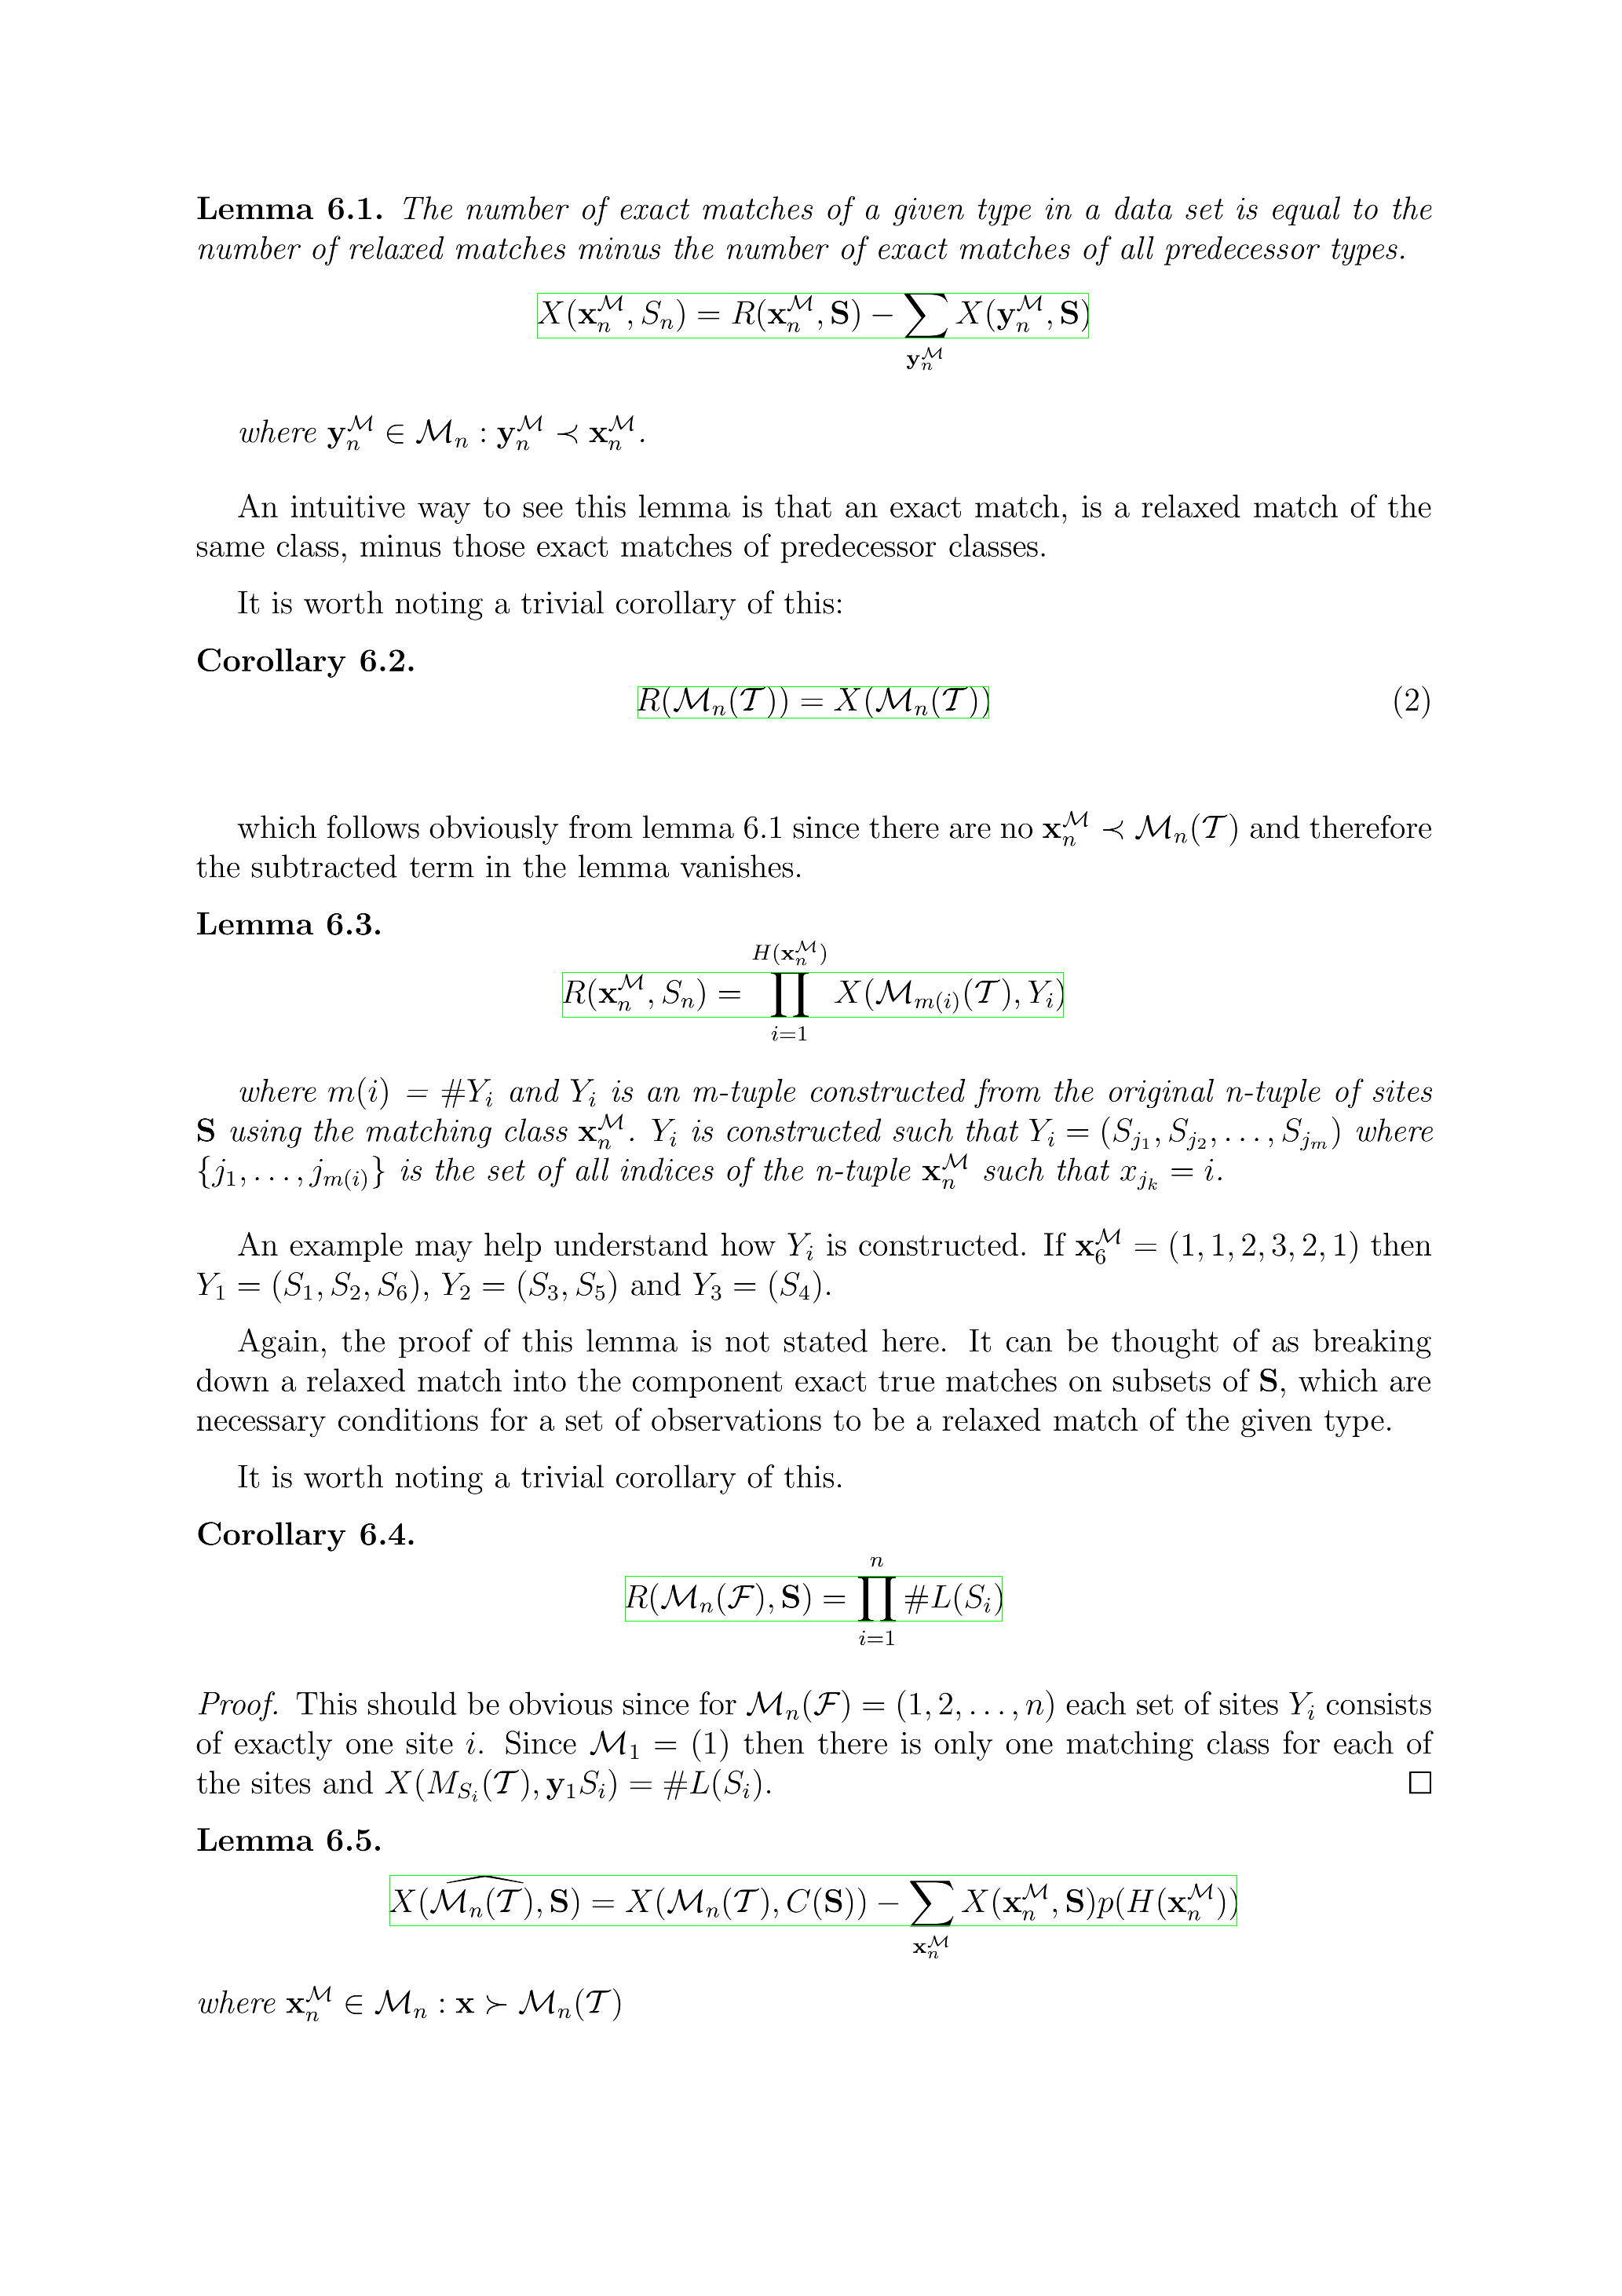
\includegraphics[width=0.42\textwidth]{result4.png} \\
 (c)  &(d)  \\
 \hline
 \end{tabular} 
 \caption{Samples of classification result }
 \label{exp_result}
\end{figure*}

\begin{table}[h]\center\scriptsize
\caption{ Summary of experimental results}
\begin{tabular}{|l|c|c|c|}\hline
                   
%$\frac{Classified as}{ Actual}  $           & Chemical & Otherl \\ \hline
%\diagdown{Classified as}{ Actual}          & Chemical & Otherl \\ \hline
%Chemical & 97.8\% & 2.2\%\\ \hline
%Non-chemical & 2.95\% & 97.05\%\\ \hline

\diaghead{\theadfont tableOfExperiment}%
{Actual}{Classified\\As}&
\thead{Chemical}&\thead{Other}\\ \hline
Chemical & 98.83\% & 1.17\%\\ \hline
Other & 1.17\% & 98.83\%\\ \hline

\end{tabular}
\label{tab:summary}
\end{table}

\subsection{Error Analysis}

\subsubsection{Classification error}
 In some cases if the operands of a chemical equation have Alkyl or Halide group, 
 they are denoted as R and X respectively. 
 But these symbols are not present in the periodic table.
 Hence, when the substrings from the OCR output are searched in the dictionary, it comes back negative.
 The equation is detected as a non-chemical one. See 4th equation bounded with a green rectangle in Fig.~\ref{cl_error}.  
\begin{figure}[h]\center\footnotesize
\begin{tabular}{|c|}
\hline
 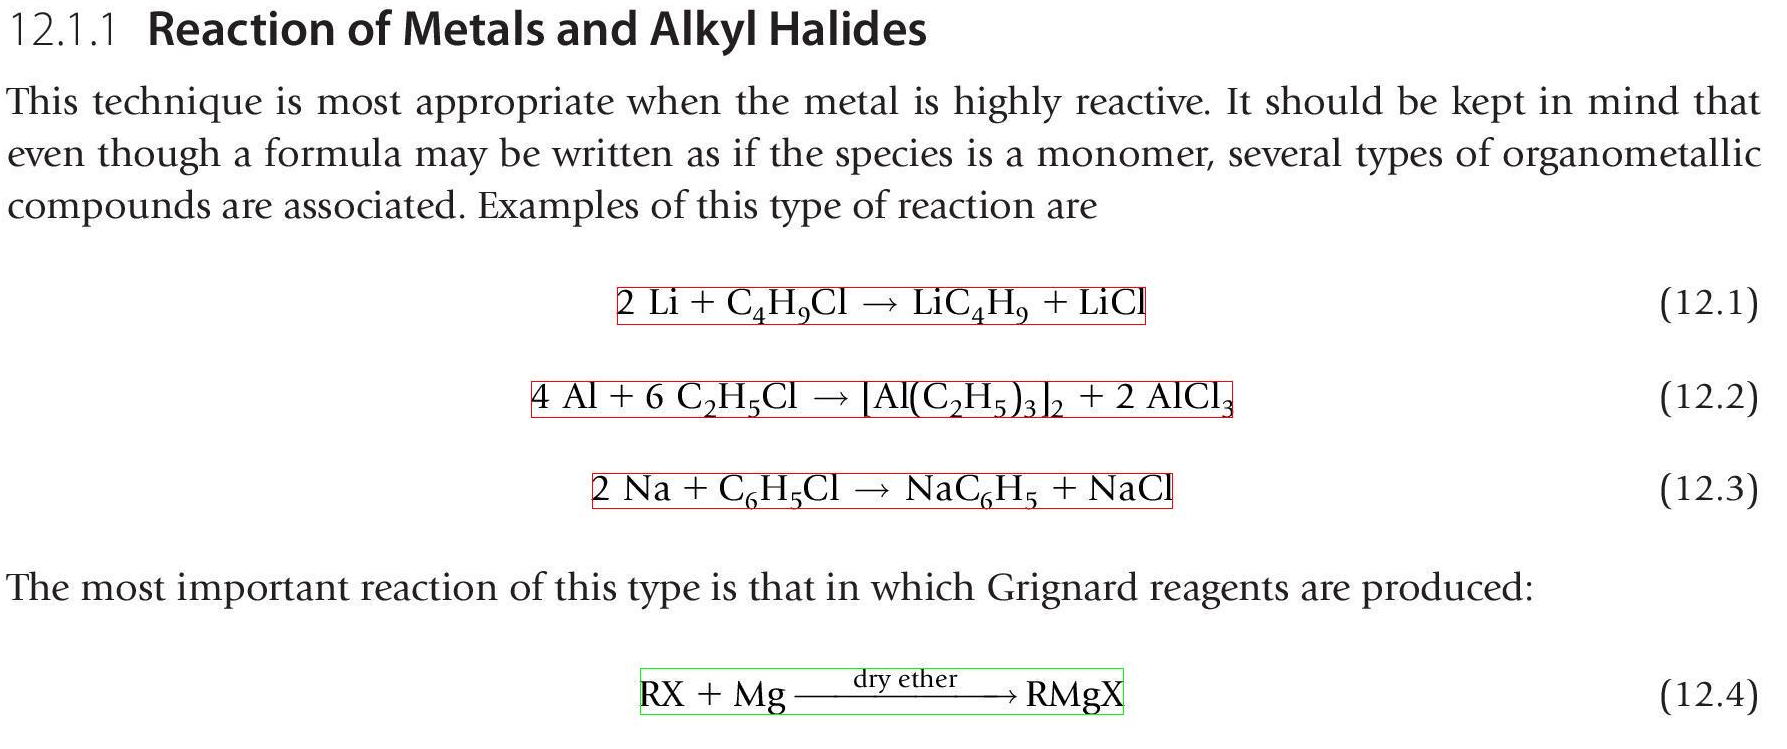
\includegraphics[width=0.42\textwidth]{cbook16.png} \\ \hline
 \end{tabular} 
 \caption{An Example of classification error.}
 \label{cl_error}
\end{figure}



\section{Auto correction of chemical compounds and the equation}

Next, auto correction is performed based on the chemical context as existing OCRs can not produce perfect result in case of chemical equations.  The output of H-RLSA  (see Fig.~\ref{h-rlsa} (d)) is taken as input here. 
Each character within a word blob is an input to the the OCR and the corresponding output  is stored in a cell and these cells form a string, S$_{chemical}$ for each word blob. For each superscript and subscript, `\^{}'  and  `\_' are inserted before them respectively in S$_{chemical}$.

 First, an error map is created based on the observation of OCR outputs of 280 chemical equations consisting of 1022 compounds (see Table \ref{table:errorTable}). Next, this table is stored into a hash map $H$ where the key is the OCR output and its value is the possible input set.
For example, if `$8$' is an erroneous OCR output for inputs `$g$', `$3$'and `$a$' (see Table \ref{table:errorTable}) then, in the hash map $H$, key is `$8$' and its corresponding value is [$g$, $3$, $a$] .

\begin{figure}[!htb]
\center\ 
\begin{tabular}{|c|} 
\hline
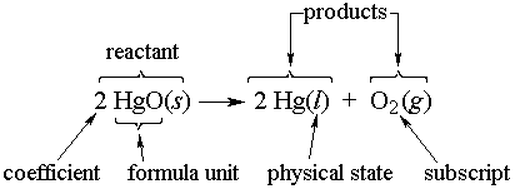
\includegraphics[width=0.5\textwidth]{chemEqParts.png}\\
\hline
\end{tabular} 
\caption{Different components of a chemical equation. }
\label{chemEqParts} 
\end{figure}  

 Each chemical compound in any equation (see Fig.~\ref{chemEqParts}) has the following format- [Coefficient]$^{[0,1]}$[Formula Unit][state]$^{[0,1]}$. Auto correction of the OCR output corresponding to each word blob includes the following steps - (i) Coefficient extraction; (ii) State separation; (iii)Auto correction of the formula unit; and (iv) Auto correction of the entire equation using Context Table.



\begin{table}[!htb]
\captionof{table}{Part of the Error list}
\begin{center}
 \begin{tabular}{|| c | c ||}
 \hline
 correct input & all observed outputs given by OCR\\
 \hline
 g & 8 S\\
 \hline
O & 0\\
\hline
3 & 8 'E s w \\
\hline
a & 3. 21 8 El 8. \\
\hline
l & 1 I\\
\hline
s & S\\
 \hline
 \end{tabular}
 \end{center}
 \label{table:errorTable}
 \end{table}




\subsection{Coefficient Extraction}

Coefficient extraction is done by matching its regular expression $[2-9]^{+}[0-9]^{*}$ at the beginning of S$_{chemical}$ as it has numerical values. 

\subsection{State separation}

  There are 4 physical states of a chemical compound which are represented by `(s)', `(g)', `(l)' and `(aq)'. To detect the physical state of the compound,  regular expression [(][A-Za-z]$^{[1,2]}$[)] is used and the checking starts from the end of S$_{chemical}$. The matched substring ($S$) is extracted from  S$_{chemical}$ and Algorithm~\ref{alg:getAllCombs} is run. 
In this algorithm, $S$ and $H$  are taken as input and all possible $Combinations$ of corrected OCR output is produced by $GetAllCombinations$ (See Fig.~\ref{stateCorrection}). These $Combinations$ are compared with `s', `g', `l' and `aq'. If no match is found, the substring extracted from S$_{chemical}$ is a radical, not a state; else, we separate the state from the compound. 

\begin{figure}[h]
\center\ 
\begin{tabular}{|c|} 
\hline
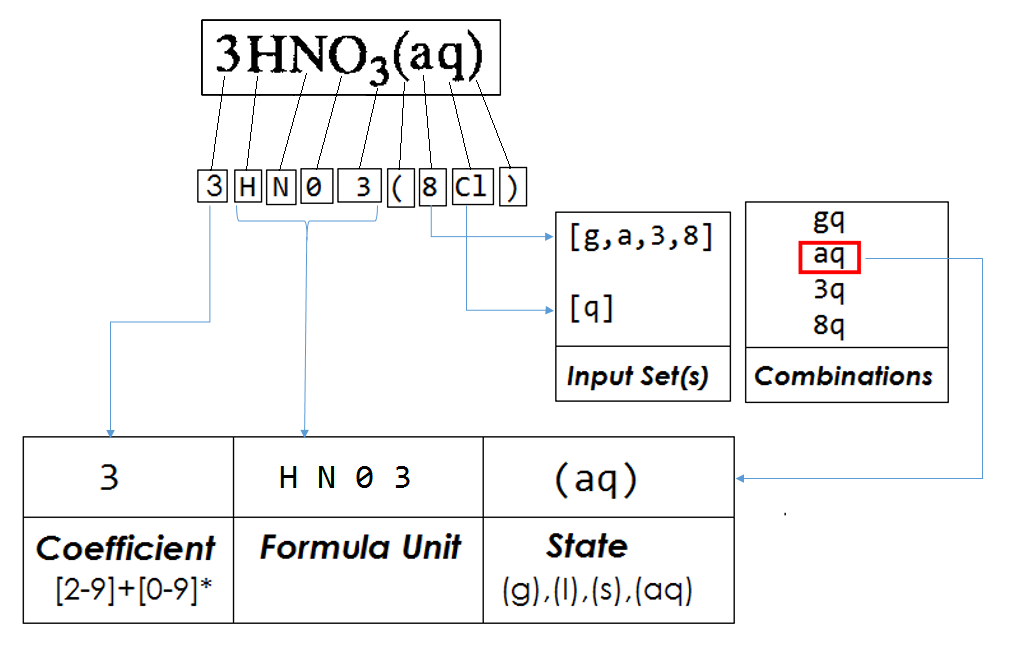
\includegraphics[width=0.5\textwidth]{stateCorrection.png}\\
\hline
\end{tabular} 
\caption{Extracting the formula unit, numeric coefficient and physical state from a chemical compound. }
\label{stateCorrection} 
\end{figure} 


\begin{algorithm}[!htb]
\large
\caption{Get All Combinations from the Error Hash Map}
\begin{algorithmic}[1]
	%\qinput{description of algorithm input}
\Procedure {GetAllCombinations}{$S$,$H$}
	%\State \textbf{Input:} {$CC, H$}
	%\State \textbf{Output:} {$Combinations$}
	\ForAll {$element(s) \in S$}
		\State $InputSet(s) \leftarrow H.Get(element)$ 
		\If {$InputSet(s)$ is $NULL$}
			\State $RETURN$ \Comment Not in Error Map
		\Else
			\If {$length(element) = 1 $}
				%\State $InputSet =\cup$  $element $
				\State $InputSets =\cup$ $[element]$ 
				\Statex \Comment Element might be correct output but still in the error list for other inputs
			\Else
				\State \textbf{Ignore}
				\Statex \Comment Input is one character, output length $>$ 1 means error
			\EndIf
		\EndIf
	\EndFor
\State $Combinations \leftarrow CartesianProduct(InputSets)$ %\Comment CartProd : Cartesian Product
\State  \textbf{Return} {$Combinations$}
\EndProcedure
\Statex
\end{algorithmic}
\label{alg:getAllCombs}
\end{algorithm}


\begin{figure}[h]
\center\ 
\begin{tabular}{|c|} 
\hline
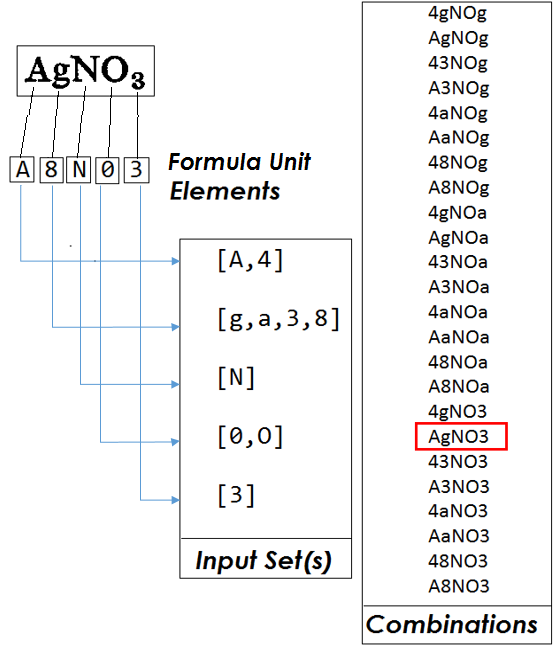
\includegraphics[width=0.5\textwidth]{autoCorrectionPictorial.png}\\
\hline
\end{tabular} 
\caption{Example of autocorrection of a formula unit. }
\label{autoCorrection} 
\end{figure} 





\subsection{Auto correction of the formula unit}

After extracting coefficient and state, only the formula unit is left in S$_{chemical}$. 
The algorithm for autocorrection of each formula unit is done in two steps (See Algorithm~\ref{alg:getAllCombs} and~\ref{alg:findMatch}). First, Algorithm~\ref{alg:getAllCombs} is performed on the formula unit.
 Next, the output of Algorithm~\ref{alg:getAllCombs}($Combinations$) are matched against a nearly exhaustive list of all molecules, chemical compounds, radicals and atoms namely $ChemList$ collected from Wikipedia \footnote{\url{http://en.wikipedia.org/wiki/Dictionary_of_chemical_formulas}}.
%( reference: %http://en.wikipedia.org/wiki/List_of_compounds). 
%% check this part
If a perfect match is found, that match is considered as the $Corrected$ formula unit (See Fig.~\ref{autoCorrection}). But in case of no match, we go for
longest common substring(s) (LCS) match ($SubMatch$).
If there is only one $SubMatch$ then the corresponding formula unit in $ChemList$ is considered as the $Corrected$  formula unit; else the $SubMatch$es are considered as $PossibleFormulaUnit$s. 



\begin{algorithm}[!htb]
\large
\caption{Find Match between ChemList and Combinations derived from Algorithm~\ref{alg:getAllCombs}}
\begin{algorithmic}[1]
\Procedure {FindMatch}{$ChemList$,$Combinations$} %\Comment $ChemList$ : nearly exhaustive list of all molecules and chemical compounds
	\ForAll{$Combinations$}
		\State \textbf{match} {with $ChemList$}
	\EndFor
	\If {\#(Match Found) = 1}
		\State $Corrected \leftarrow Match$
		\State  \textbf{Return} {$Corrected$}
	\ElsIf {\#(Match Found) = 0}
		\State $SubMatch \leftarrow \textbf{LCS}(Combinations,ChemList)$ 
		\Statex \Comment LCS : Longest Common Substring
		\If {{NumberOf}($SubMatch$)=1}
			\State $Corrected \leftarrow SubMatch$
			\State  \textbf{Return} {$Corrected$}
		\Else
			\State $PossibleFormulaUnit(s) \leftarrow SubMatch$
			\State  \textbf{Return} {$PossibleFormulaUnit(s)$}
		\EndIf
	\Else
		\State $PossibleFormulaUnits \leftarrow Matches$
		\State  \textbf{Return} {$PossibleFormulaUnit(s)$}
		\Statex \Comment Multiple matches
	\EndIf
\EndProcedure
\end{algorithmic}
\label{alg:findMatch}
\end{algorithm}


\subsection{Auto correction of the entire equation using Context Table}

Here, we have all the possible formula units and try to find out the $FinalEquation$ in the context of the equation itself. Algorithm~\ref{alg:alg3} takes all $Corrected$ and $PossibleFormulaUnit$s and returns the $FinalEquation$ by forming the Context Table. 
Chemical equations have the same periodic elements in the left hand side, called $Reactants$ as that in the right hand side, called $Products$. All the periodic elements follow the regular expression [A-Z][a-z]*. So, for each  $PossibleFormulaUnit$, the set of periodic elements in the $Reactants$, $P_{R}$ and in the $Products$, $P_{P}$ are computed and stored in the $Context Table$. When the set difference of $P_{R}$ and $P_{P}$ in the table is empty, that $PossibleFormulaUnit$ is considered as $Corrected$ and included in the $FinalEquation$ (See Fig.~\ref{context}). But if the above condition comes true for multiple possibilities, we cannot decide which of the possible formula units are actually in the original equation.The algorithm shows multiple $FinalEquation$s. This is considered an $ERROR$ case.
An example of formation of context table is demonstrated in  Fig.~\ref{context}. The co-effiecient and state (if any) are added with their correspodning $Corrected$ formula unit. The $FinalEquation$ is then converted to \LaTeX\  format using $mhchem$ package.

\begin{algorithm}[!htb]
\large
\caption{Auto-Correction of the entire equation using chemical context table}
\begin{algorithmic}[1]
\Procedure {GetFinalEqn}{$PossibleFormulaUnit$,$Corrected$}
	\State {Include all $Corrected$ units in $FinalEquation$}
	\State{$Count  \leftarrow 0$}
	\For{every $PossibleFormulaUnit$}
		\State \textbf{compute}($P_{R}$)  
		\Statex \Comment{$P_{R}$ :  Set of periodic elements in Reactants}
		\State \textbf{compute}($P_{P}$)  \
		\Statex \Comment {$P_{P}$ : Set of periodic elements in Products}
		
		\If{$P_{R} - P_{P} = \emptyset $}
			\State $Corrected \leftarrow PossibleFormulaUnit$
			\State {Include that in the $FinalEquation$}
			\State $Count \leftarrow Count + 1$
		\EndIf
	\EndFor
	\If {$Count \geq 2 $}
		\State {Multiple $Corrected$ compounds}
		\State{Multiple $FinalEquations$}
		\Statex \Comment { $ERROR$}
	\EndIf
	\State  \textbf{Return} {$FinalEquation(s)$}
\EndProcedure
\end{algorithmic}
\label{alg:alg3}
\end{algorithm}

\begin{figure}[!htb]
\center\ 
\begin{tabular}{|c|} 
\hline
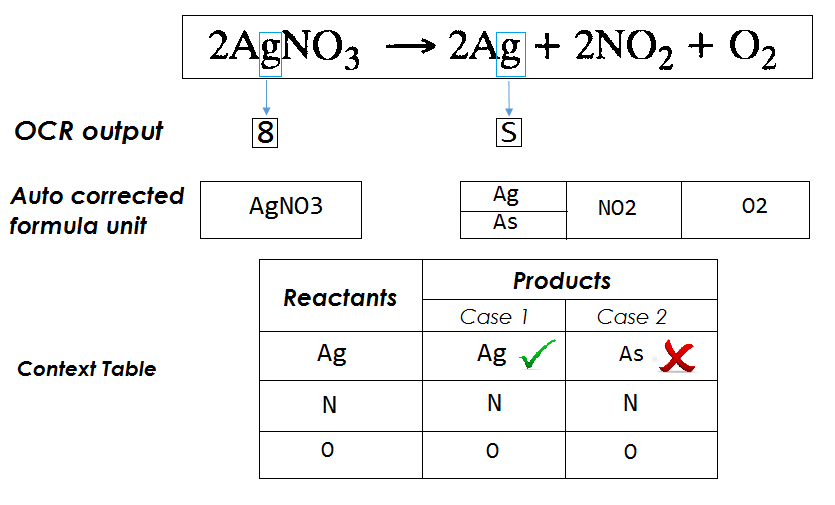
\includegraphics[width=0.5\textwidth]{equationContext.png}\\
\hline
\end{tabular} 
\caption{Formation of context table. }
\label{context} 
\end{figure}


\subsection{Experimental Result}
\label{sc_exp_res}

We have implemented our algorithm in MATLAB 8.3.0.532
(R2014a) in a PC (Intel(R) Core(TM) i5-3337U CPU @ 1.80GHz
running Windows 8). The proposed method has been tested on
a dataset consisting 234 document pages. Out of 234 pages 50
pages are taken from ICDAR 2013 Math-zone segmentation
datasets and other document pages are scanned from different Mathematics and
Chemistry books. 
The summary of the experimental results
is shown in Table~\ref{table:result}. Out of 3406 chemical compounds in the test dataset, 114 were partially corrected and 52 could not be corrected at all. The overall accuracy of autocorrection is 95.12\%. These results are quite encouraging. See the sample image (Fig.~\ref{eg}(a)). Corresponding segmented displayed chemical equations are shown in Fig.~\ref{eg}(b). Fig.~\ref{eg}(c) shows the direct OCR output where `i' has been wrongly identified as `l', `I' and `1' (for $Si$ in all the lines of  Fig.~\ref{eg}(c)). Similarly `O' results in `0' (line 1,2,3). `S' sometimes is detected as `5' (line 5). Our auto correction algorithm remedies these issues. Fig.~\ref{eg}(d) demonstrates the effect of our auto correction algorithm. This algorithm is targeted towards chemical equation with linear representation. More results are included in the following website \url{https://sites.google.com/site/chemeqndb/}

\begin{figure}[!htb]
\center\footnotesize
\begin{tabular}{ |c|c|}
\hline
 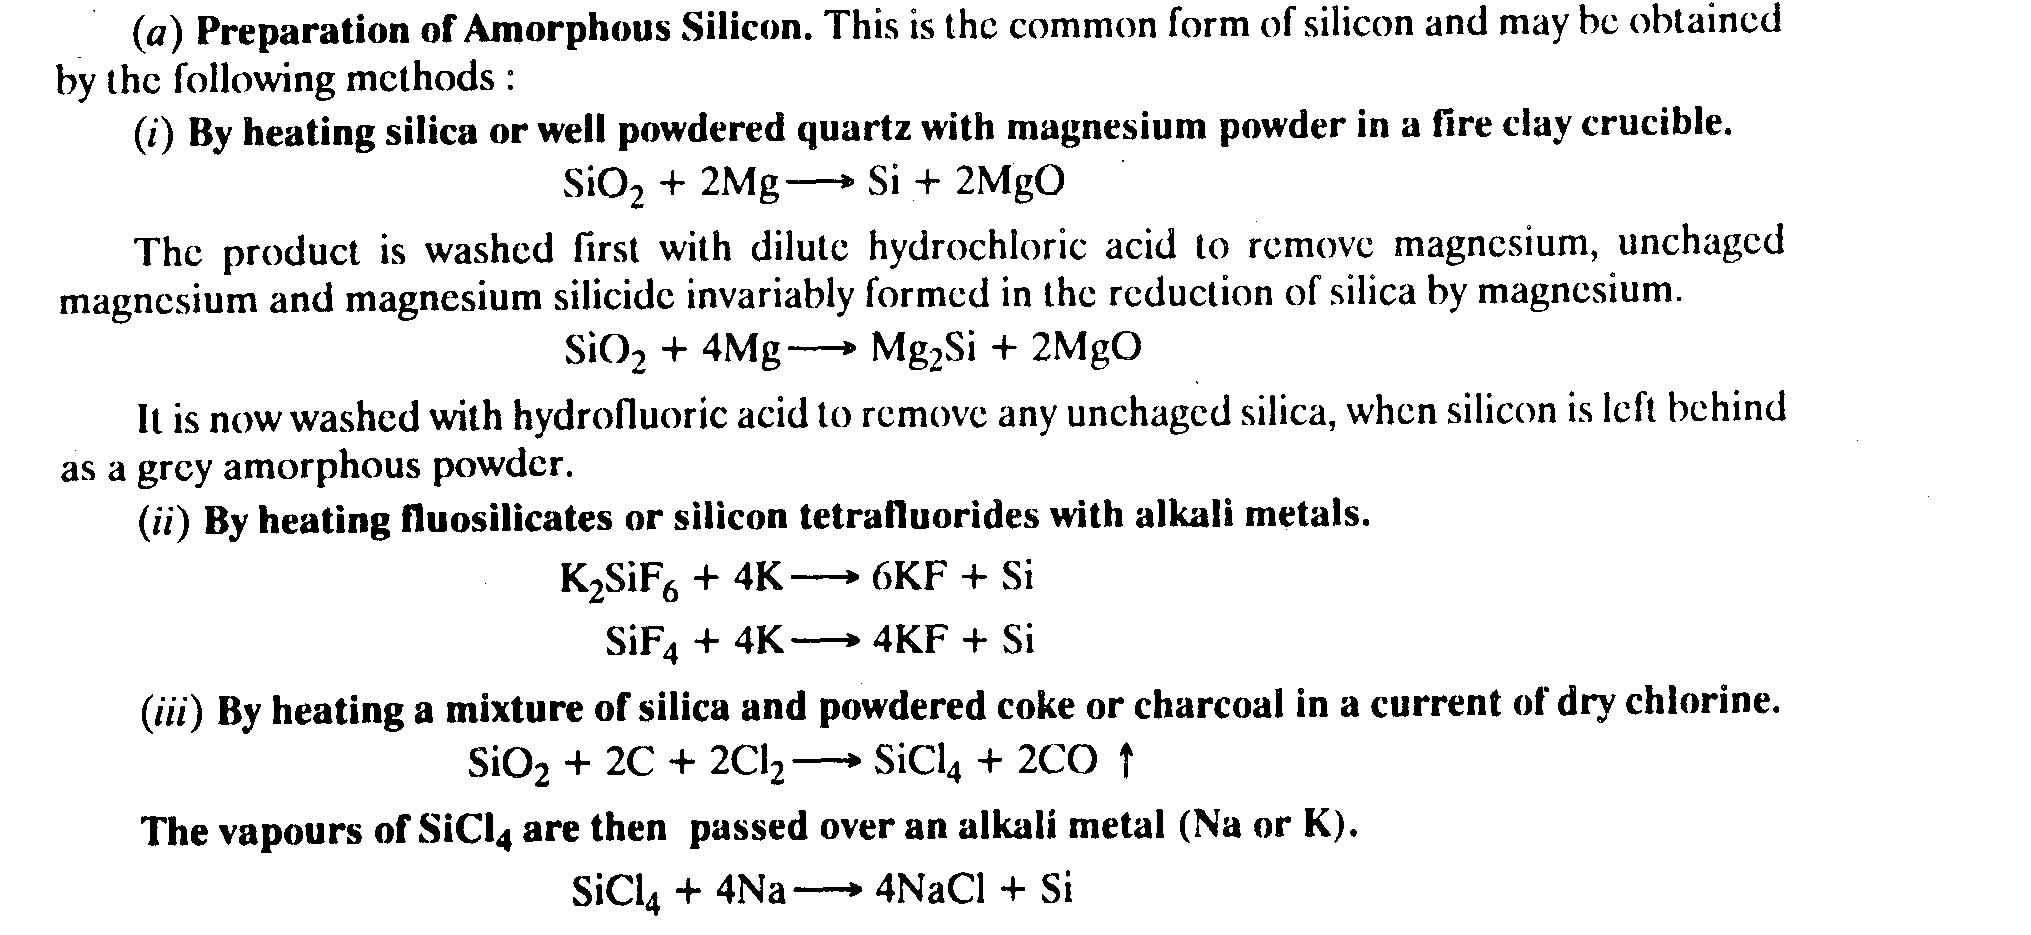
\includegraphics[width=0.28\textwidth]{sampleDocument.png} &
 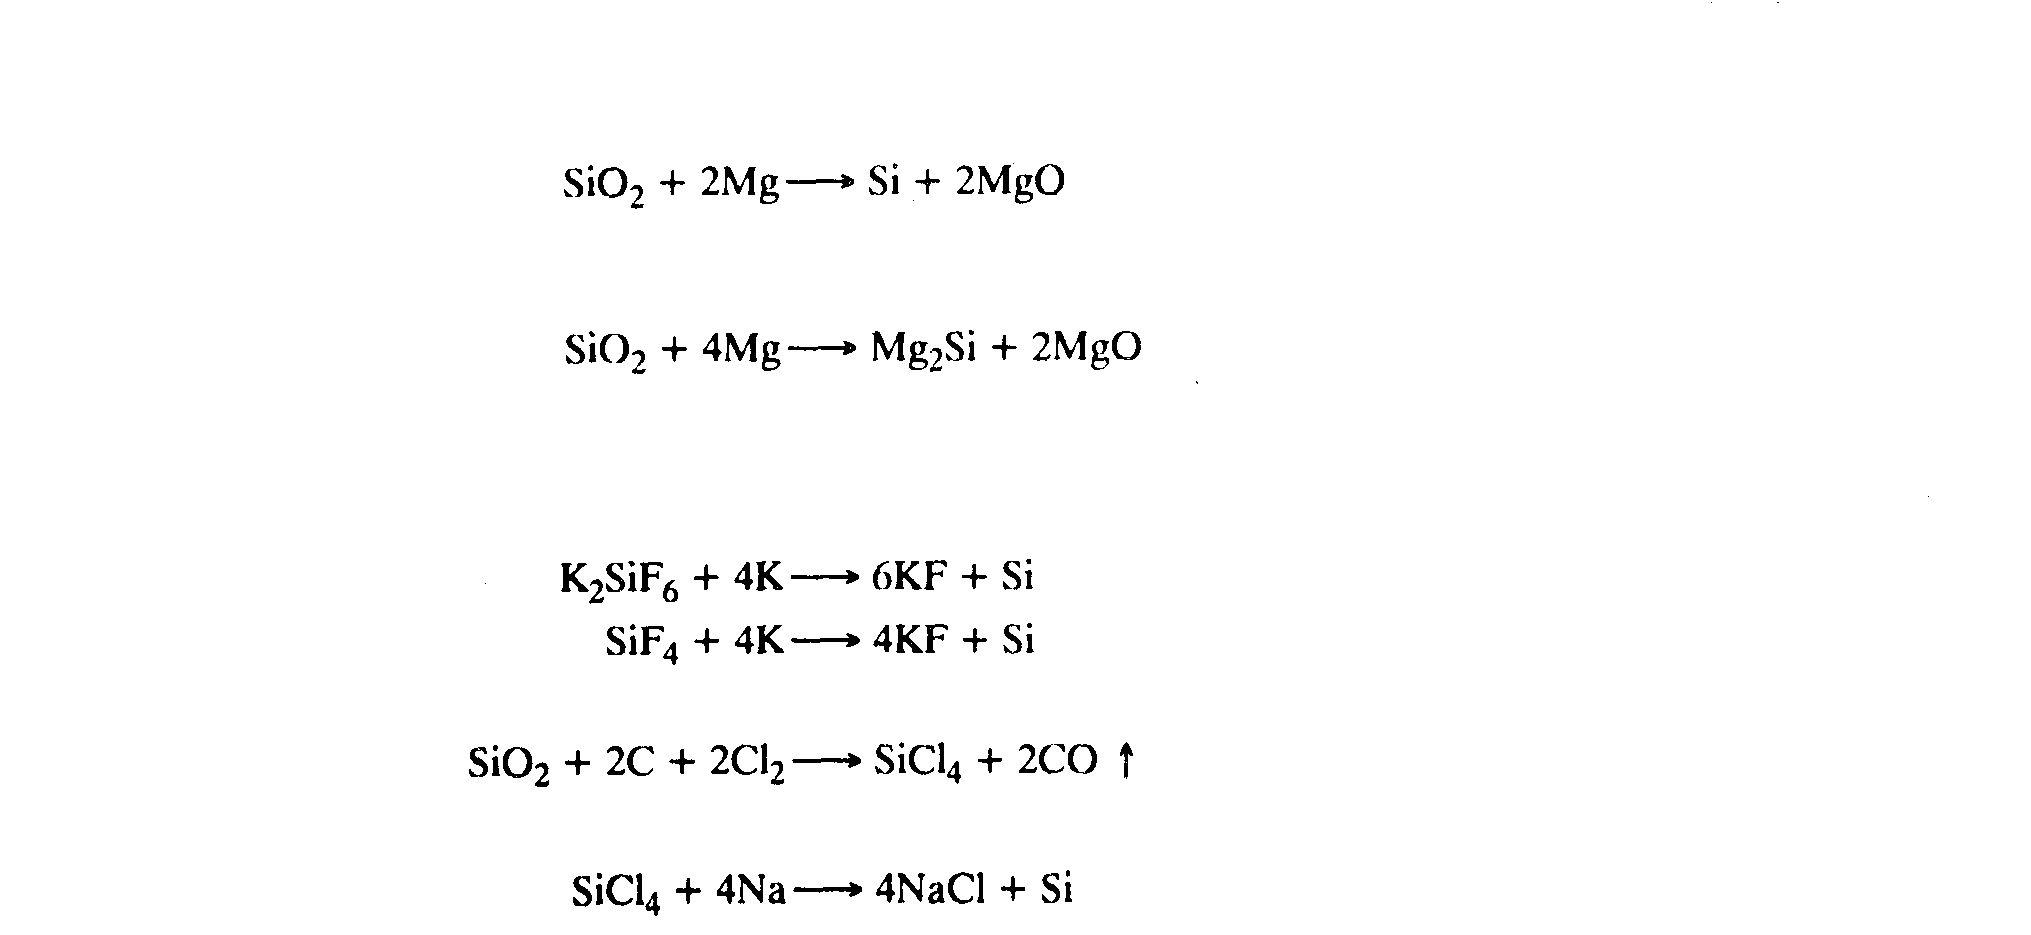
\includegraphics[width=0.28\textwidth]{DCE.png} \\
(a)  & (b) \\ 
%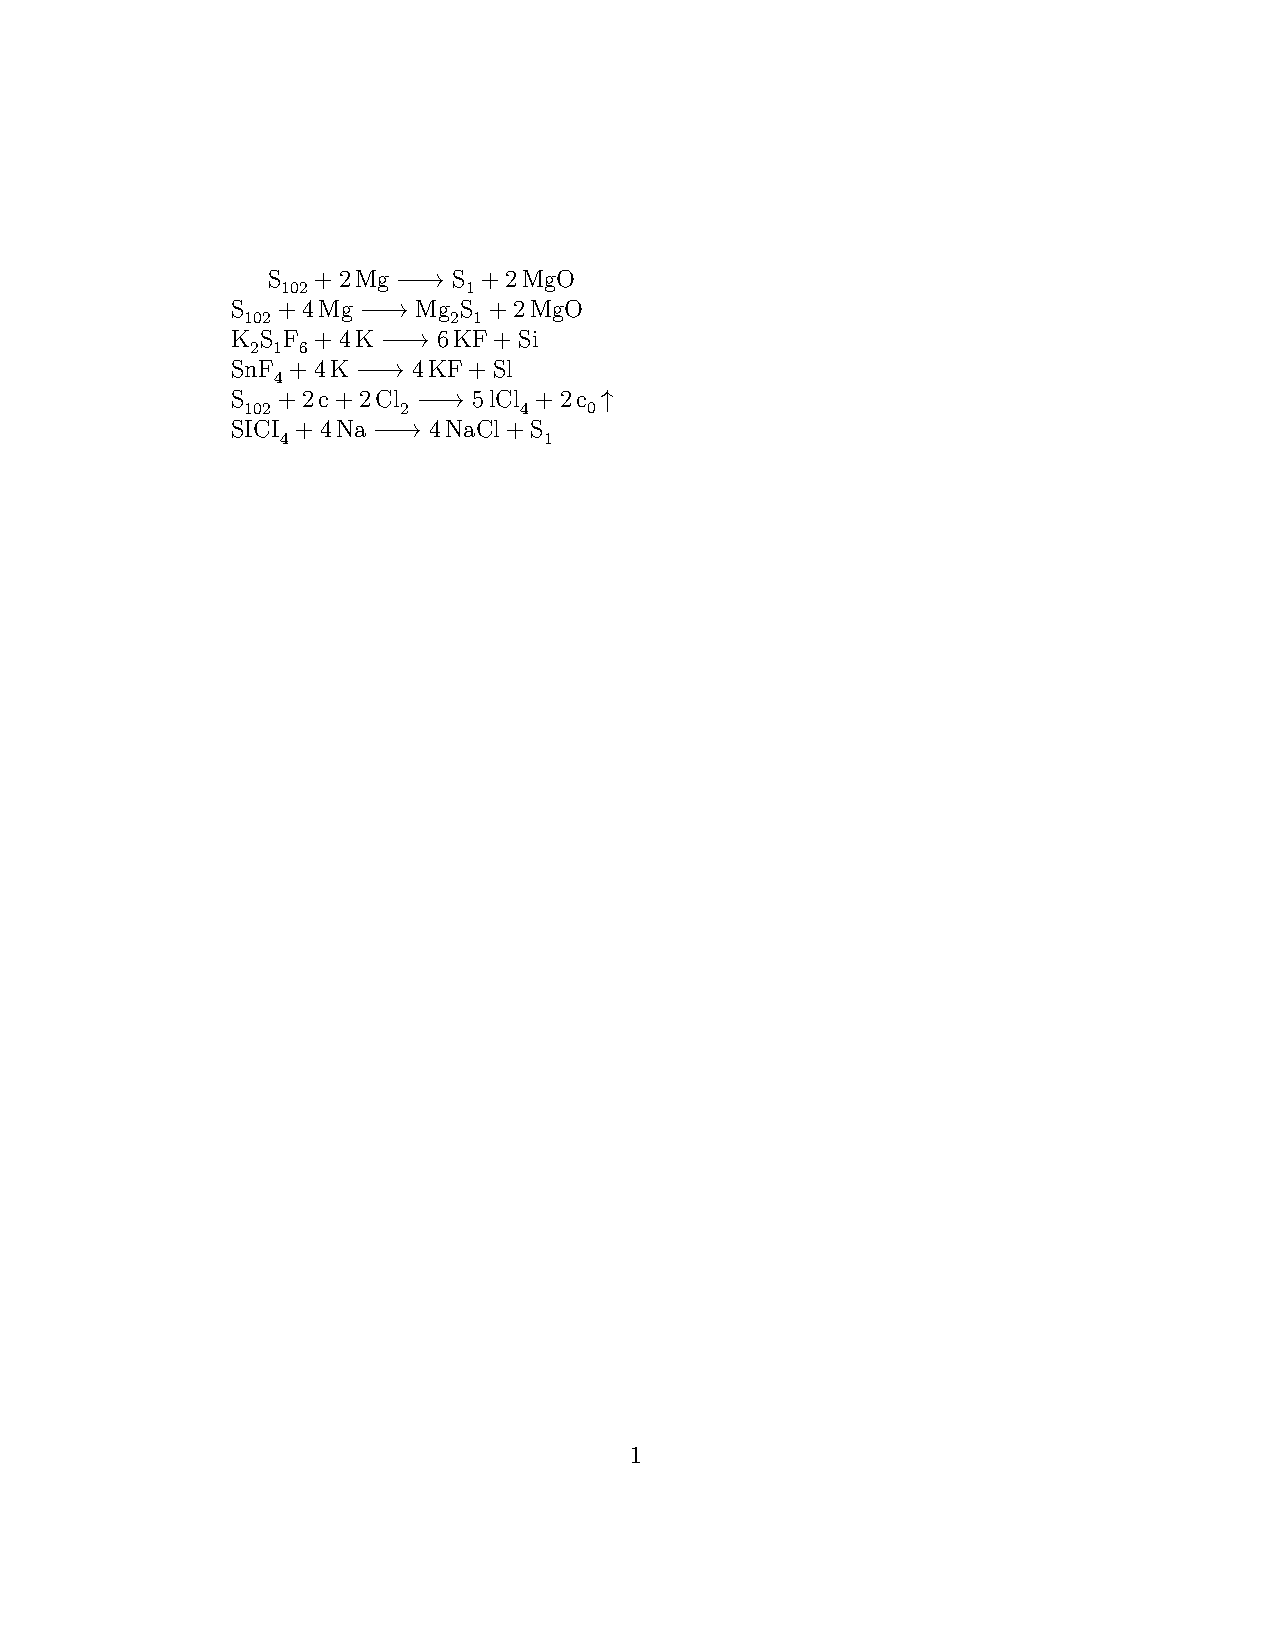
\includepdf[(pages={1})]{ directOCR.pdf } \\
\hline
 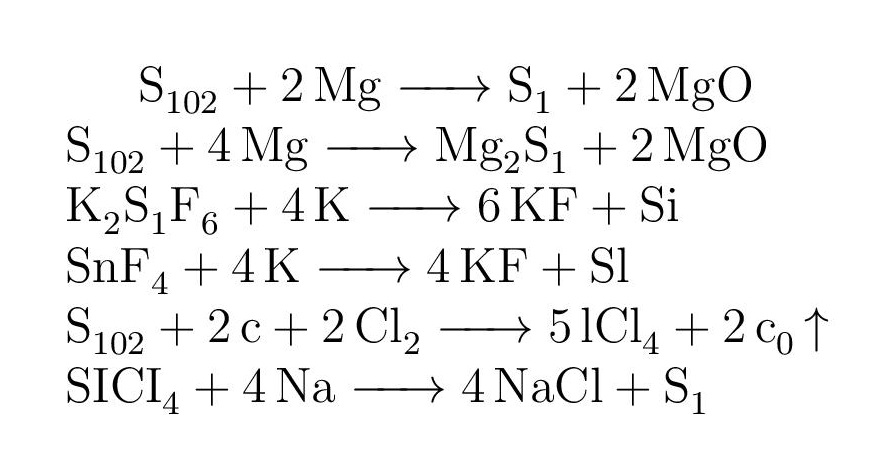
\includegraphics[width=0.28\textwidth]{directOCR.jpg} &
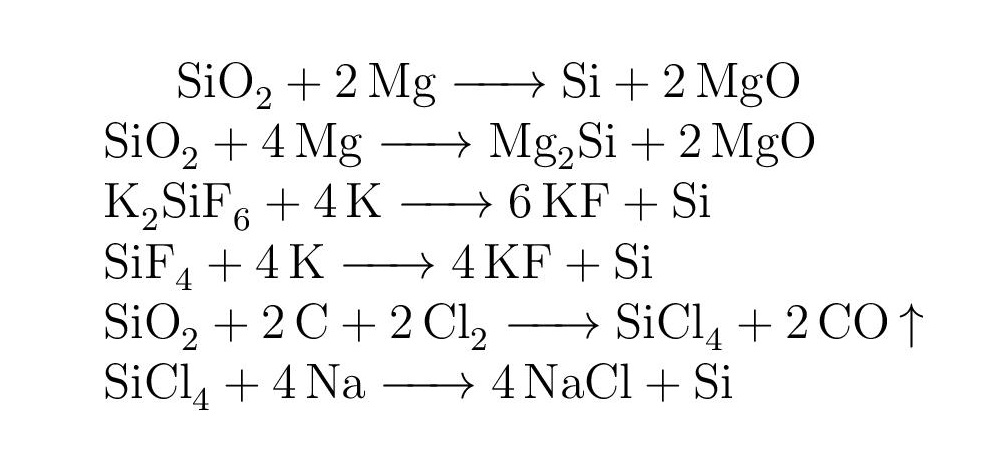
\includegraphics[width=0.28\textwidth]{correctedFinalEq.jpg}\\
 
 (c)  & (d)  \\
 \hline
\end{tabular}
\caption{Experimental result; (a) Input image; (b) Segmented Chemical equation;
(c) OCR output in PDF format; (d) Output of the proposed method.}
\label{eg} 
\end{figure}


\begin{table}[!htb]
\captionof{table}{Summary of Experimental Results}
\centering
\begin{tabular}{|c|c|}
\cline{1-2} 
{\color[HTML]{000000} \# Total Images}                     & 234   \\ 	\cline{1-2}
{\color[HTML]{000000} \# Total Chemical Operands}                        & 3460    \\ \cline{1-2}
{\color[HTML]{000000} DE segmentation accuracy}            & 95.12\% \\ \cline{1-2}
\end{tabular}
\label{table:result}
\end{table}


\subsection{Error Analysis}
Here we try to analyse the sources of some of the errors which have negative effect on the performance figures both for segmentation and classification.

\subsubsection{Auto Correction Error}
The Auto Correction Algorithm fails when the chemical equation contains some text such as $and$, $or$ etc between two displayed equation in the same line. Also, when the chemical compound is written in formats such as $(Na_2SiO_3)_n$, only $Na_2SiO_3$ is detected based on $ChemList$. Some equations have conditions (pressure, temperature) written over the arrows. We have not ventured in that yet. But the error case that has been mentioned in Algorithm~\ref{alg:alg3} has very less probability of occurrence. Hence it is ignored.


\chapter{Conclusion}
\label{sc_conclu}
We have presented an automated chemical equation segmentation and chemical context based auto correction system that is able to provide the exact searchable format of linear chemical equations in any document image.  
The method is based on detecting operators as +, - and $ \rightarrow$ which are common in both chemical and non-chemical equations,
segmenting the displayed equations and then running them through an open source OCR to classify.
A publicly available database for mathematical documents and scanned images of various chemistry 
books in  both English and Bengali language are used in this study. 
The experimental results demonstrate the efficiency of our proposed method. 
The present work points to several new research avenues to be explored further. 
The over-all performance itself demands further research in this area. Excessive degradation due to aging and
improper digitization of the document images give rise to broken and merged characters which give conflicting output
from the OCR. In the future, design of a better integrated OCR specifically for
chemical equations would be ventured in.
In addition, formation of  ``electron bond matrix"  of a chemical compound in a reaction mentioned in 
the introduction chapter would be a high-level goal in the future.
Auto correction on non-linear or bond structure representations of chemical equations could be ventured in.


%%%%%%%%%%%%%%%%%%%%%%%%%%%%%%%%%%%%%%%%
\begin{thebibliography}{1}
\bibitem{blostein_97}
 D. Blostein and A. Grabavec.
\newblock {\em ``Recognition of Mathematical Notation'',}
\newblock {\em Handbook of Character Recognition and document Image Analysis}, 557--582, 1997.

\bibitem{chan_2000}
K-F. Chan and D-Y. Yeung.
\newblock {\em``Mathematical Expression Recognition: A Survey''.}
\newblock {\em IJDAR, Vol. 3, no, 1}, 3--15, 2000.

\bibitem{Garain_07}
U. Garain and B. B. Chaudhuri.
\newblock {\em On OCR of Printed mathematical Expressions.}
\newblock {\em ``Digital Document Processing'',Ed. B. B. Chaudhuri, Advances in pattern 
Recognition}, 235--259 , 2007.

\bibitem{fateman_96}
\newblock R. Fateman, T. Tokuyasu, B. Berman, and N. Mitchell.
\newblock {\em ``Optical character recognition and parsing of typeset mathematics'',
Visual Commun. And Image Representation, Vol 7, no 1}, 2--15, 1996.

\bibitem{toumit_99}
\newblock J. Y. Toumit, S. Garcia-Salicetti, and H. Emptoz.
\newblock {\em ``A hierarchical and recursive model of mathematical expressions for
automatic reading of mathematical documents''. In Proc. of
ICDAR}, 116--122, 1999.
 
\bibitem{kacem_01}
\newblock A. Kacem, A. Beliad and M. Ben Ahmed.
\newblock {\em ``Automated Extraction of printed mathematical formulas using fuzzy logic
and propagation of context'', IJDAR, vol.4 no. 2}, 97--108, 2001.

\bibitem{suzuki_03}
\newblock M. Suzuki, F. Tamari, R. Fukuda, S. Uchida and T. Kanahori.
\newblock {\em ``INFTY - An Integrated OCR system for Mathematical Documents'', Proc. of 
ACM Symposium on Document Engineering}, 95--104, 2003.

\bibitem{Garain_09}
\newblock Utpal Garain.
\newblock {\em `` Identification of Mathematical Expressions in Document Images'',
Proc. of ICDAR}, 1340--1344, 2009.

\bibitem{Garain_05}
\newblock Utpal Garain.
\newblock {\em ``Recognition of Printed Handwritten Mathematical Expressions'', Ph.D Thesis,
ISI, Kolkata, India}, 2005.

\bibitem{Garain_01}
\newblock B. B. Chaudhuri and U. Garain.
\newblock {\em ``Extraction of type atyle based meta-information from Imaged
documents'', IJDAR, vol. 3 no. 3}, 138--149, 2001.

\bibitem{jin_03}
\newblock J. Jin, X. Han and Q. Wang.
\newblock {\em ``Mathematical formulas extraction'', Proc. of ICDAR}, 1138--1141, 2003.

\bibitem{drake_05}
\newblock D. M. Drake and H. S. Baird.
\newblock {\em ``Distinguishing mathematical notation from english text
using computational geometry'', Proc. of ICDAR}, 1270--1274, 2005.

\bibitem{guo_07}
\newblock Y.-S. Guo, L. Huang and C.-P. Liu.
\newblock {\em ``A new approach for understanding of structure of printed mathematical
expressions'', Proc. of ICMLC}, 2633--2638, 2007.

\bibitem{liu_13}
\newblock We-Te Chu and Fan liu.
\newblock {\em ``Mathematical formula detection from heterogeneous document
Images'', Proc. of CTAAI}, 140--146, 2013.

\bibitem{skm_07}
S. P. Chowdhury, S. Mandal, A. K. Das, and B. Chanda.
\newblock {\em ``Segmentation of Text and Graphics from Document Images''},
\newblock in {\em Proc. of ICDAR}, 619--623, 2007.

\bibitem{gonzalez92}
R.~C.~Gonzalez and R.~Woods.
\newblock {\em ``Digital Image Processing''}.
\newblock Addision-Wesley, 1992.

\bibitem{skm_06}
S. Mandal, S. P. Chowdhury, A. K. Das, and B. Chanda,
\newblock {\em ``A simple and effective table detection system from Document Images''},
\newblock in {\em Proc. of IJDAR, Vol. 8(2)}, 172--182, 2006.

\bibitem{spc_07} S.~P.~Chowdhury, S.~Mandal, A.~K.~Das, and
B.~Chanda, \emph{Segmentation of Text and Graphics from Document
Images}, In Proc. of ICDAR, pp. 619–623,2007.

\bibitem{sekhar_06} S.~Mandal, S.~P.~Chowdhury, A.~K.~Das, and
B.~Chanda, \emph{A simple and effective table detection system
from Document Images}, IJDAR, Vol. 8(2), 172–182, 2006.

\bibitem{blostein_97} D.~Blostein and A.~Grabavec,
\emph{Recognition of Mathematical Notation}, Handbook of
Character Recognition and document Image Analysis, 577--582,
1997.
 
\bibitem{chan_00} K-F.~Chan and D-Y.~Yeung, \emph{Mathematical
Expression Recognition: A Survey}, IJDAR, Vol. 3, no: 1, 3–15,
2000.

\bibitem{Garain_07} U.~Garain and B.~B.~Chaudhuri \emph{An OCR
of Printed mathematical Expressions, Digital Document
Processing}, Ed: B.~B.~Chaudhuri, Advances in pattern
Recognition, 235–259 , 2007.

\bibitem{uchid_10}
A.~Fujiyoshi, M.~Suzuki, S.~Uchid,
 \emph{Grammatical Verification for Mathematical Formula Recognition Based on Context-Free Tree Grammar},
 Mathematics in Computer Science, 279--298, 2010.
 
 
 \bibitem{algorri_07}
 M.~E.~Algorri, M.~Zimmermann, C.~M.~Friedrich, S.~Akle, and M.~Hofmann-Apitius,
\emph{Reconstruction of chemical molecules from images},
In Proc. 29th Annual International IEEE Conference on Engineering in
Medicine and Biology Society, 4609--4612, 2007.

\bibitem{algorri_07a}
M.~E.~Algorri, M.~Zimmermann, and M.~Hofmann-Apitius,
\emph{Automatic recognition of chemical images},
In pro. Eighth Mexican International Conference on Current Trends in Computer Science, 41--46, 2007.
\bibitem{park_09}
J.~Park, G.~R.~Rosania, K.~A.~Shedden, M.~Nguyen, N.~Lyu, and K.~Saitou,
\emph{Automated extraction of chemical structure information from digital raster images}, Chemistry Central journal, vol. 3(1), 2009.
\end{thebibliography}



\end{document}